\chapter{Kinematic reweighting in the gluino search}
\label{app:meffrw}

In this appendix we discuss in more details the kinematic reweighting mentioned in Section \ref{sec:strong:dataMC},
designed to mitigate the effect of the mismodeling that affects all the energy-related variables in the 1-lepton channel,
where we observe a downward trend in the data/MC ratio, clearly visible e.g. in the bottom panel of 
Figure \ref{fig:strong:datamc:meff_prerw_1L}; 
this does not happen instead in the 0-lepton channel, as it can be observed in 
Figure \ref{fig:strong:datamc:meff_prerw_0L}.
This difference in trends is problematic for the analysis, since all of the \glspl{vr} require at least one signal lepton, 
including the ones used to derive the prediction for 0-lepton \glspl{sr}.

To have a better estimate of the background in the high-$\meff$ regime, a reweighting has been derived to bring the MC prediction closer to the observed data. This reweighting is computed in a region that requires:
\begin{itemize}
\item at least 4 jets,
\item exactly 2 $b$-jets,
\item $\met$ $>$ 200 GeV,
\item at least one lepton,
\item $\mtb$ $<$ 140 GeV.
\end{itemize}

This selection is orthogonal to \glspl{sr} and \glspl{cr} but has a similar background composition. 
The $\mtb$ selection reduces further the signal contamination and allows for a validation region with exactly 2 $b$-jets and high $\mtb$. 
The same trend in the data/MC ratio in the \meff distribution has been observed also in other regions non dominated by the 
\ttbar background,
therefore the reweighting is computed taking into account all backgrounds and applied to all backgrounds. 
The binning of the reweighting is chosen to be 50 GeV for most of the \meff spectrum, 
while at high \meff the width of the bins is larger to allow $\approx$ 100 data events in each bin. 
Before deriving the reweighting, the sum of the \gls{mc} predictions for the different backgrounds is scaled to the same yield as in data,
so that the reweighting.
The final reweighting for the 1-lepton channel is shown in the bottom panel of Figure \ref{fig:meff_in2b_no_corr}.

\begin{figure}[htbp]
\centering
\subfigure[]{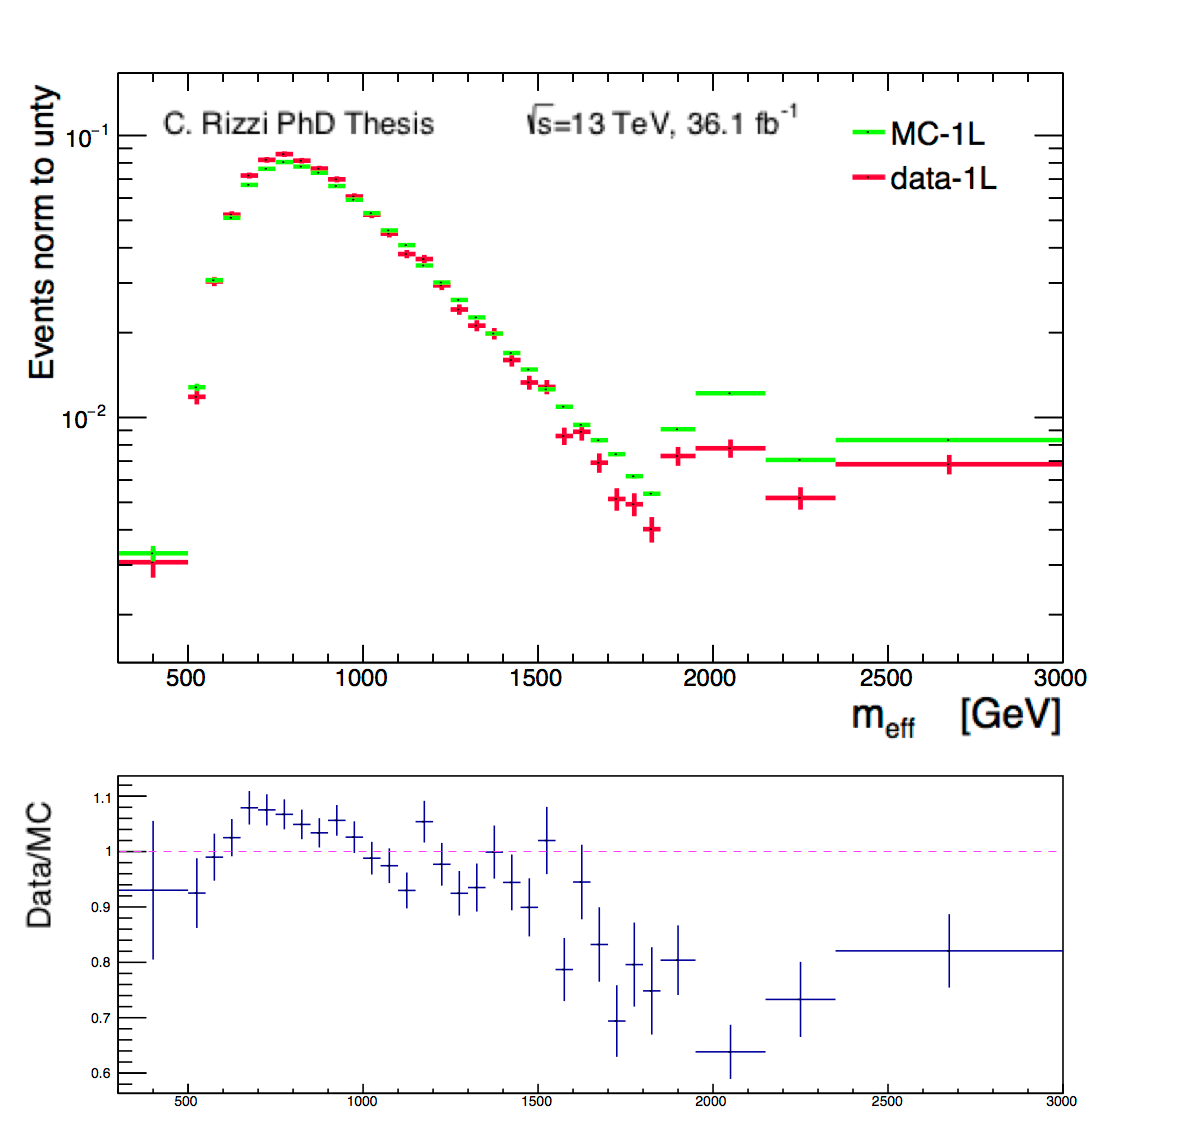
\includegraphics[width=0.55\textwidth]{figures/App1/Rizzi-FigA1-1-1.pdf}}
\caption{$\meff$ distribution in data and simulation in a selection that requires at least 4 jets, exactly 2 $b$-jets, $\met$ $>$ 200 GeV,
at least one lepton, and $\mtb$ $<$ 140 GeV.}
\label{fig:meff_in2b_no_corr}
\end{figure}

\section{Effect on other variables}

Figures \ref{fig:strong:rwCR::datamc1L_a}--\ref{fig:strong:rwCR::datamc1L_d}
show the effect of the reweighting on the main kinematic variables.
We can see that the reweighting, derived using only the \meff distribution, improves the 
comparison between data and the simulation 
in most of the energy-related variables.

\begin{figure*}[htbp]
\centering 
\subfigure[\meff, before reweighting]{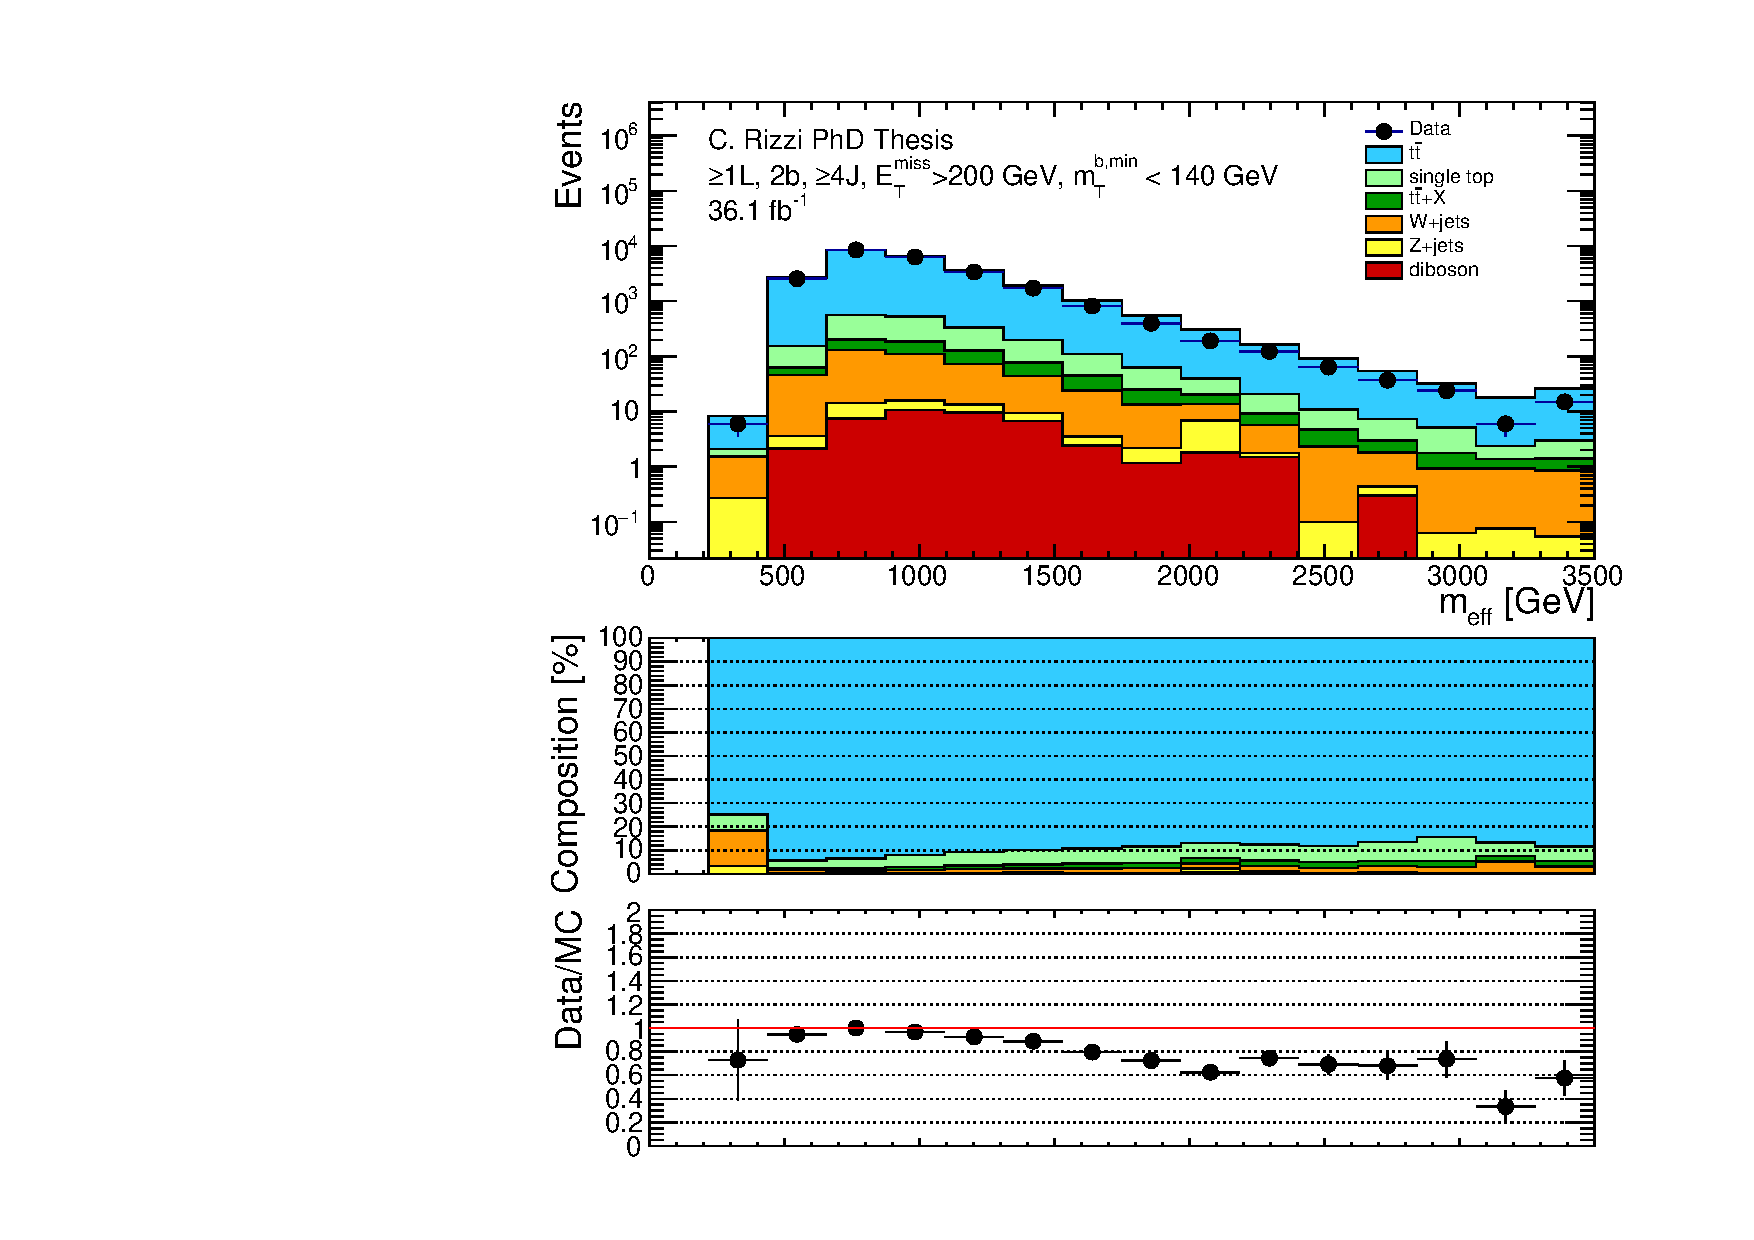
\includegraphics[width=0.45\textwidth]{figures/App1/Rizzi-FigA1-2-1.pdf}
\label{fig:strong:rwCR::datamc1L:meff_incl}}
\subfigure[\meff, after reweighting]{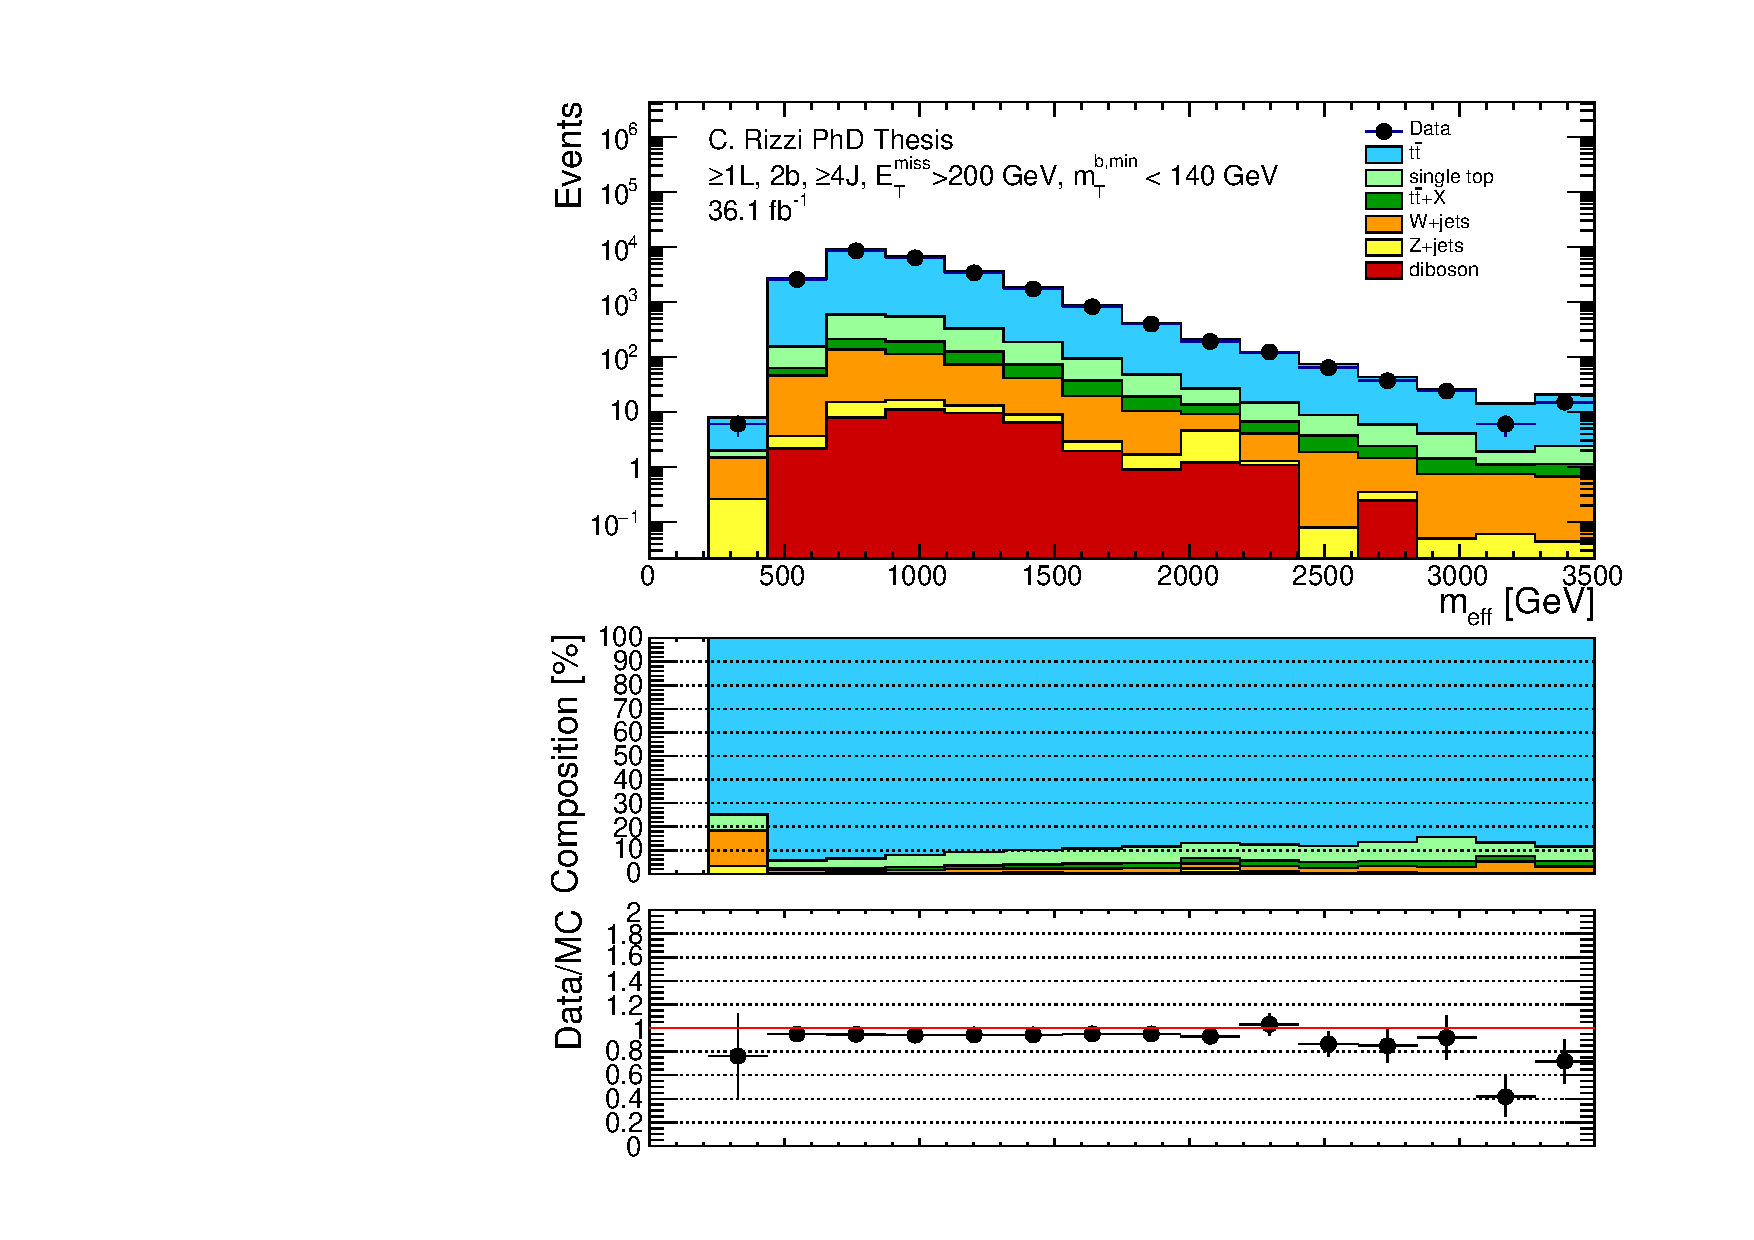
\includegraphics[width=0.45\textwidth]{figures/App1/Rizzi-FigA1-2-2.pdf}
\label{fig:strong:rwCR::datamc1L:meff_incl}}\\
\subfigure[\mjsum, before reweighting]{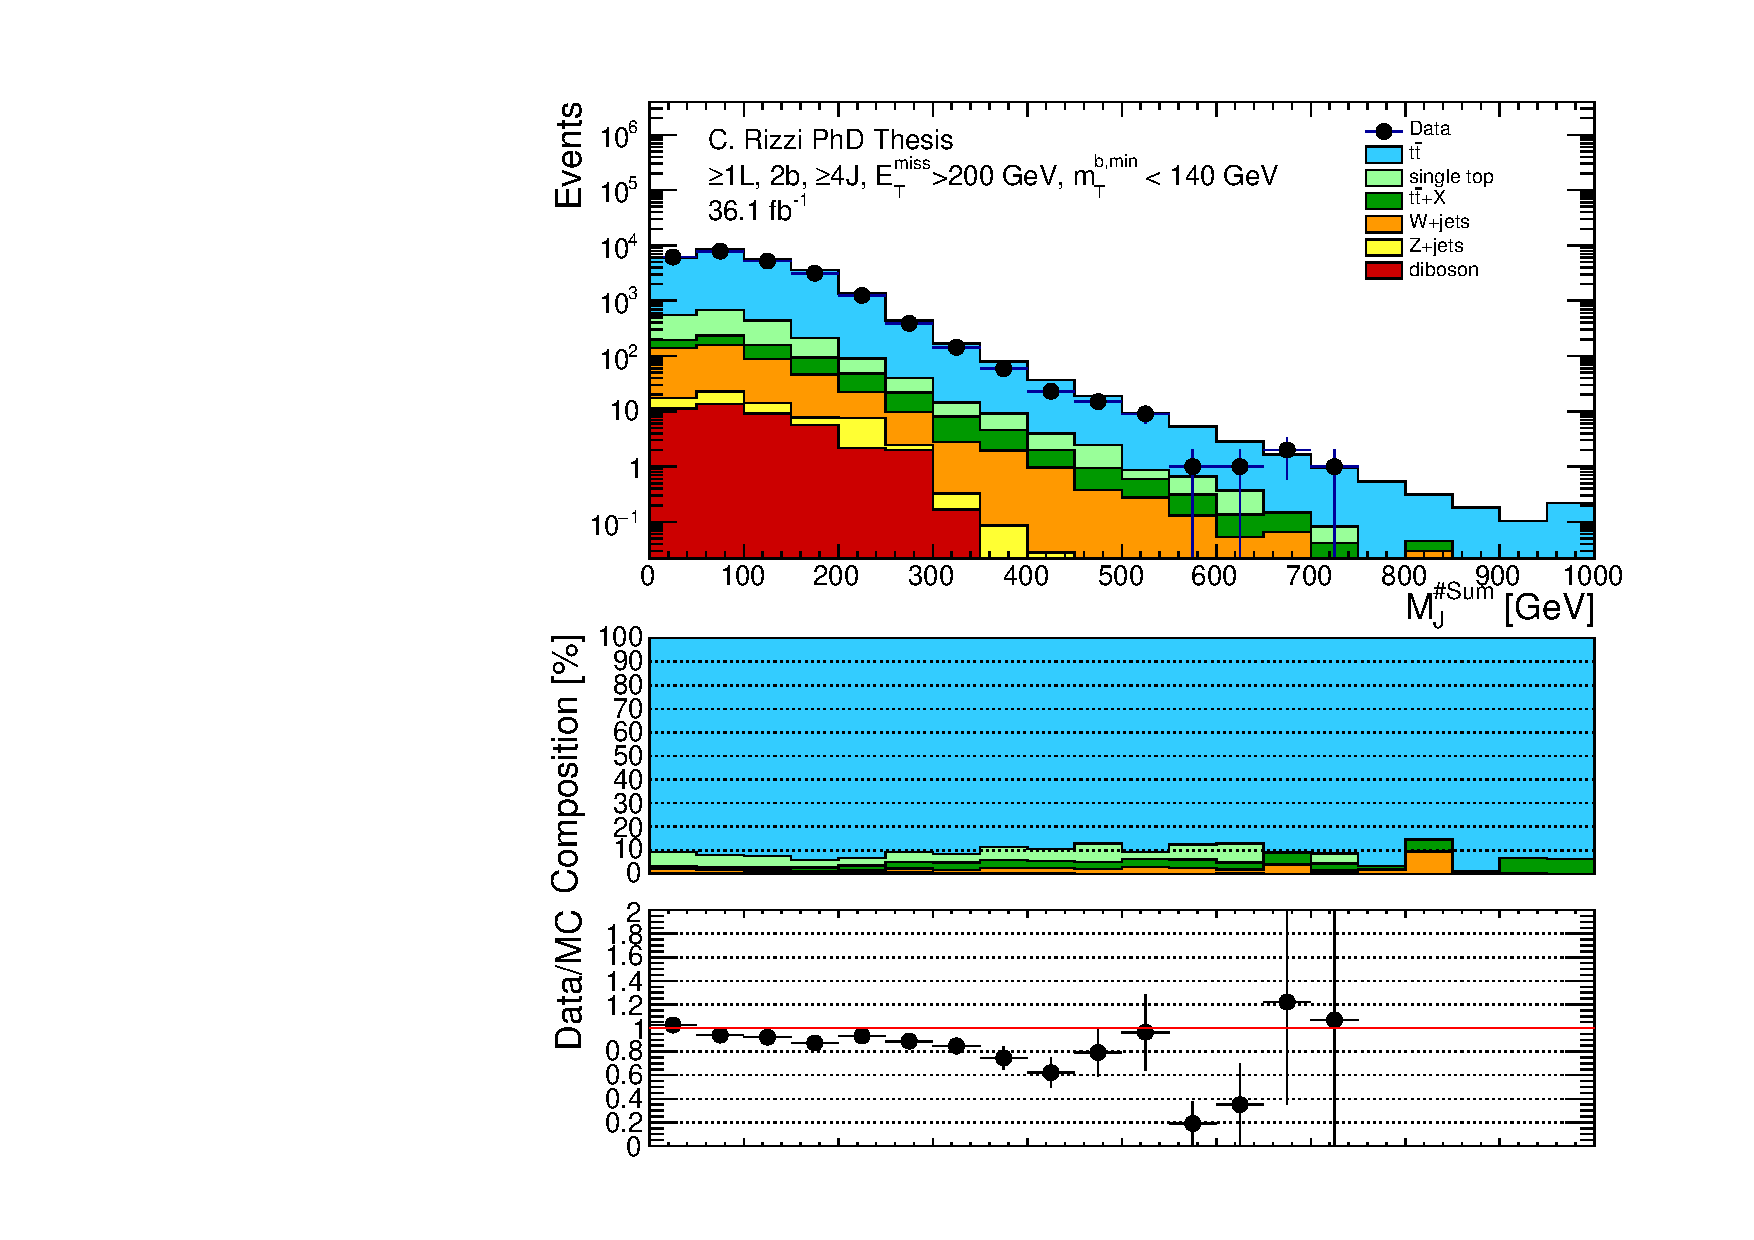
\includegraphics[width=0.45\textwidth]{figures/App1/Rizzi-FigA1-2-3.pdf}
\label{fig:strong:rwCR::datamc1L:MJSum_rc_r08pt10}}
\subfigure[\mjsum, after reweighting]{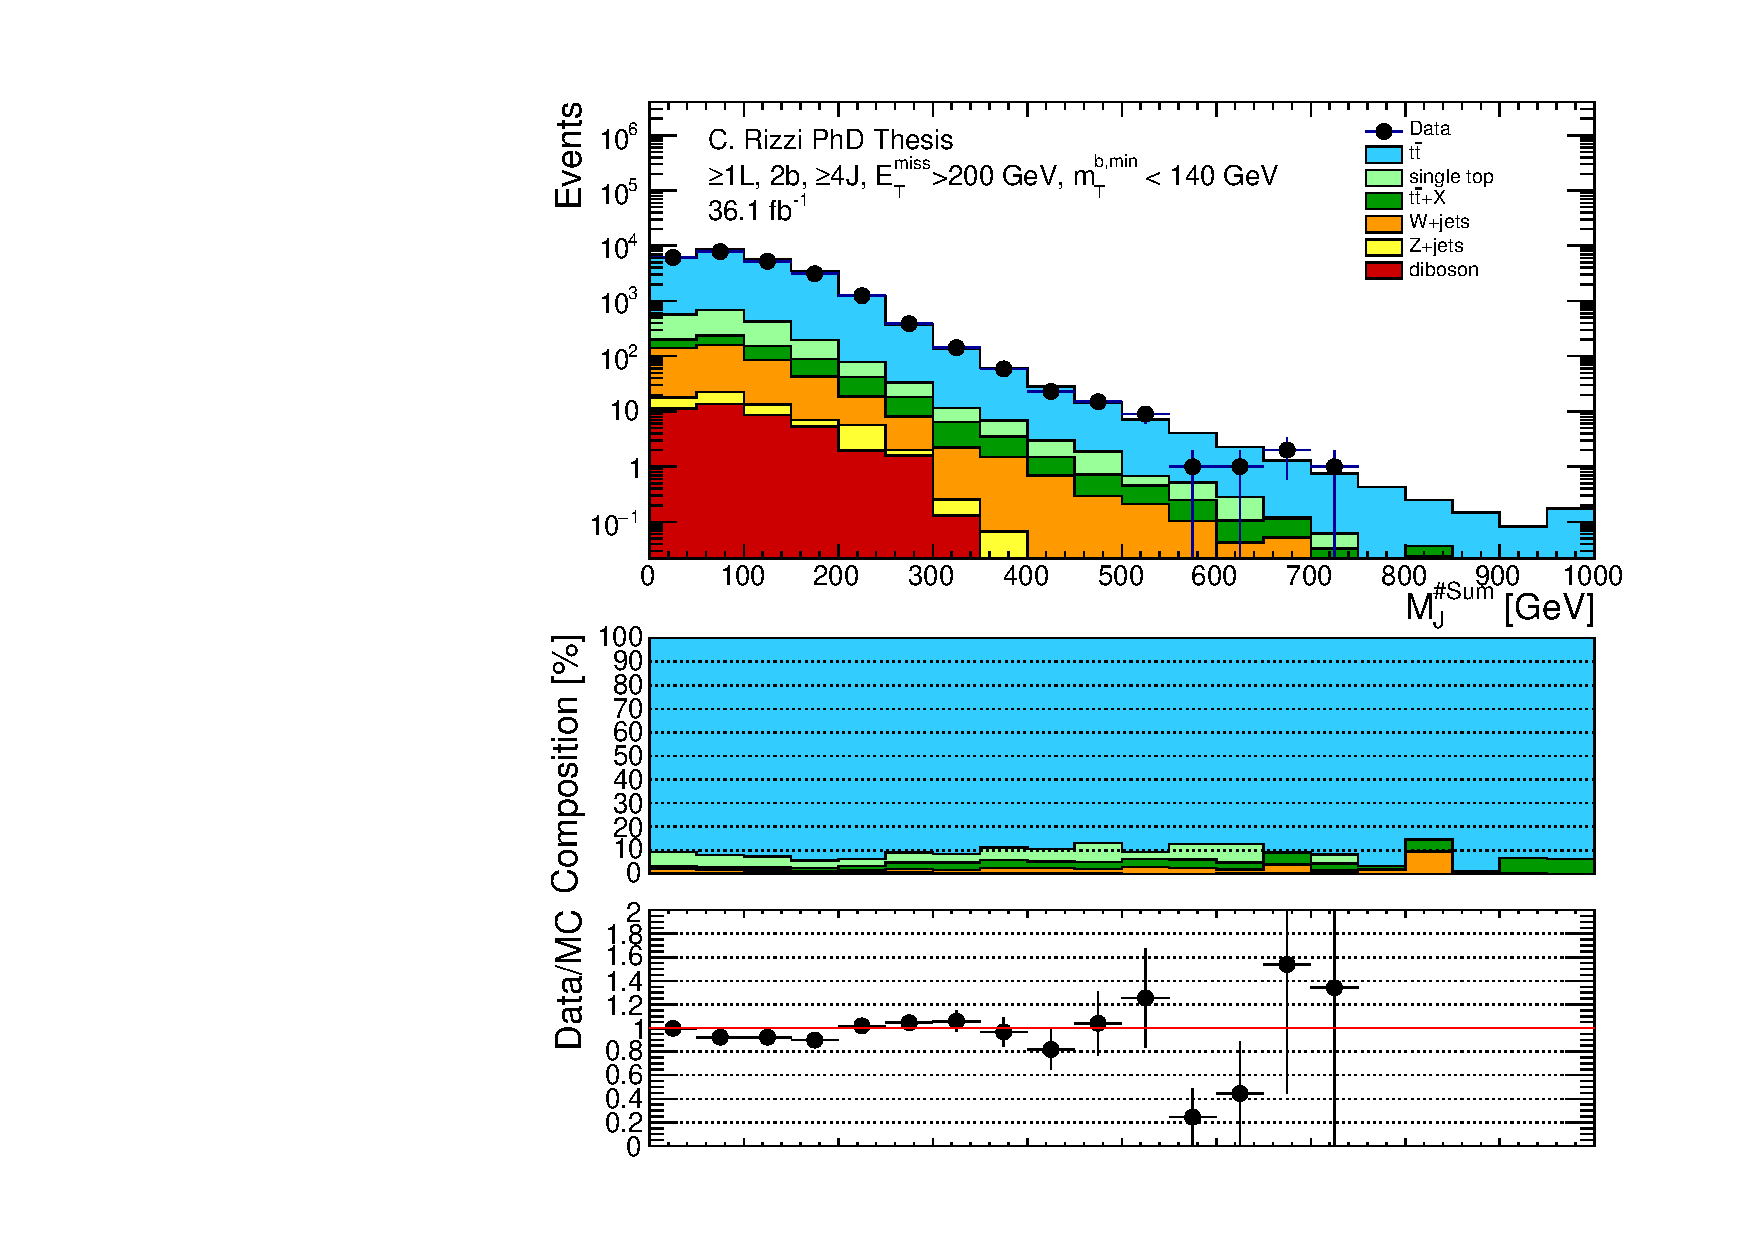
\includegraphics[width=0.45\textwidth]{figures/App1/Rizzi-FigA1-2-4.pdf}
\label{fig:strong:rwCR::datamc1L:MJSum_rc_r08pt10}}\\
\subfigure[\met, before reweighting]{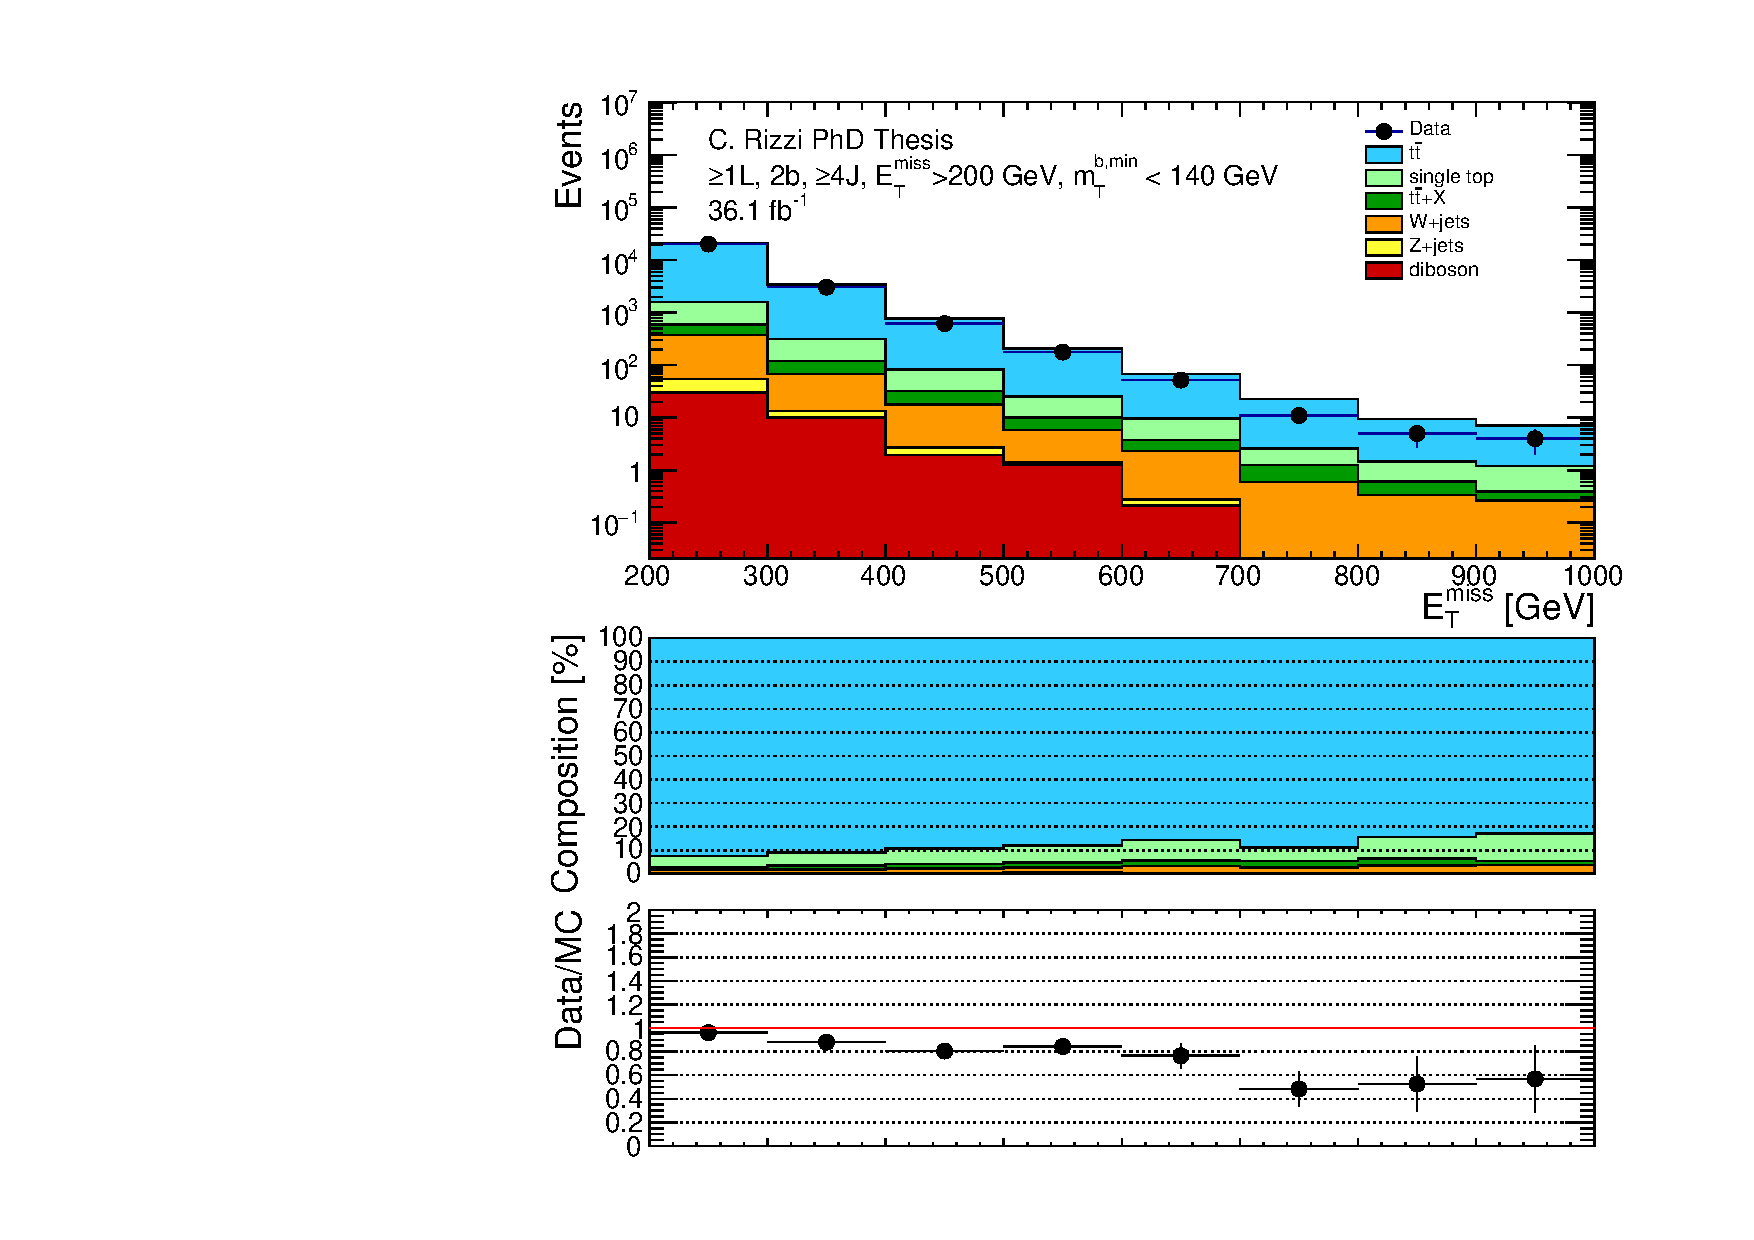
\includegraphics[width=0.45\textwidth]{figures/App1/Rizzi-FigA1-2-5.pdf}
\label{fig:strong:rwCR::datamc1L:met}}
\subfigure[\met, after reweighting]{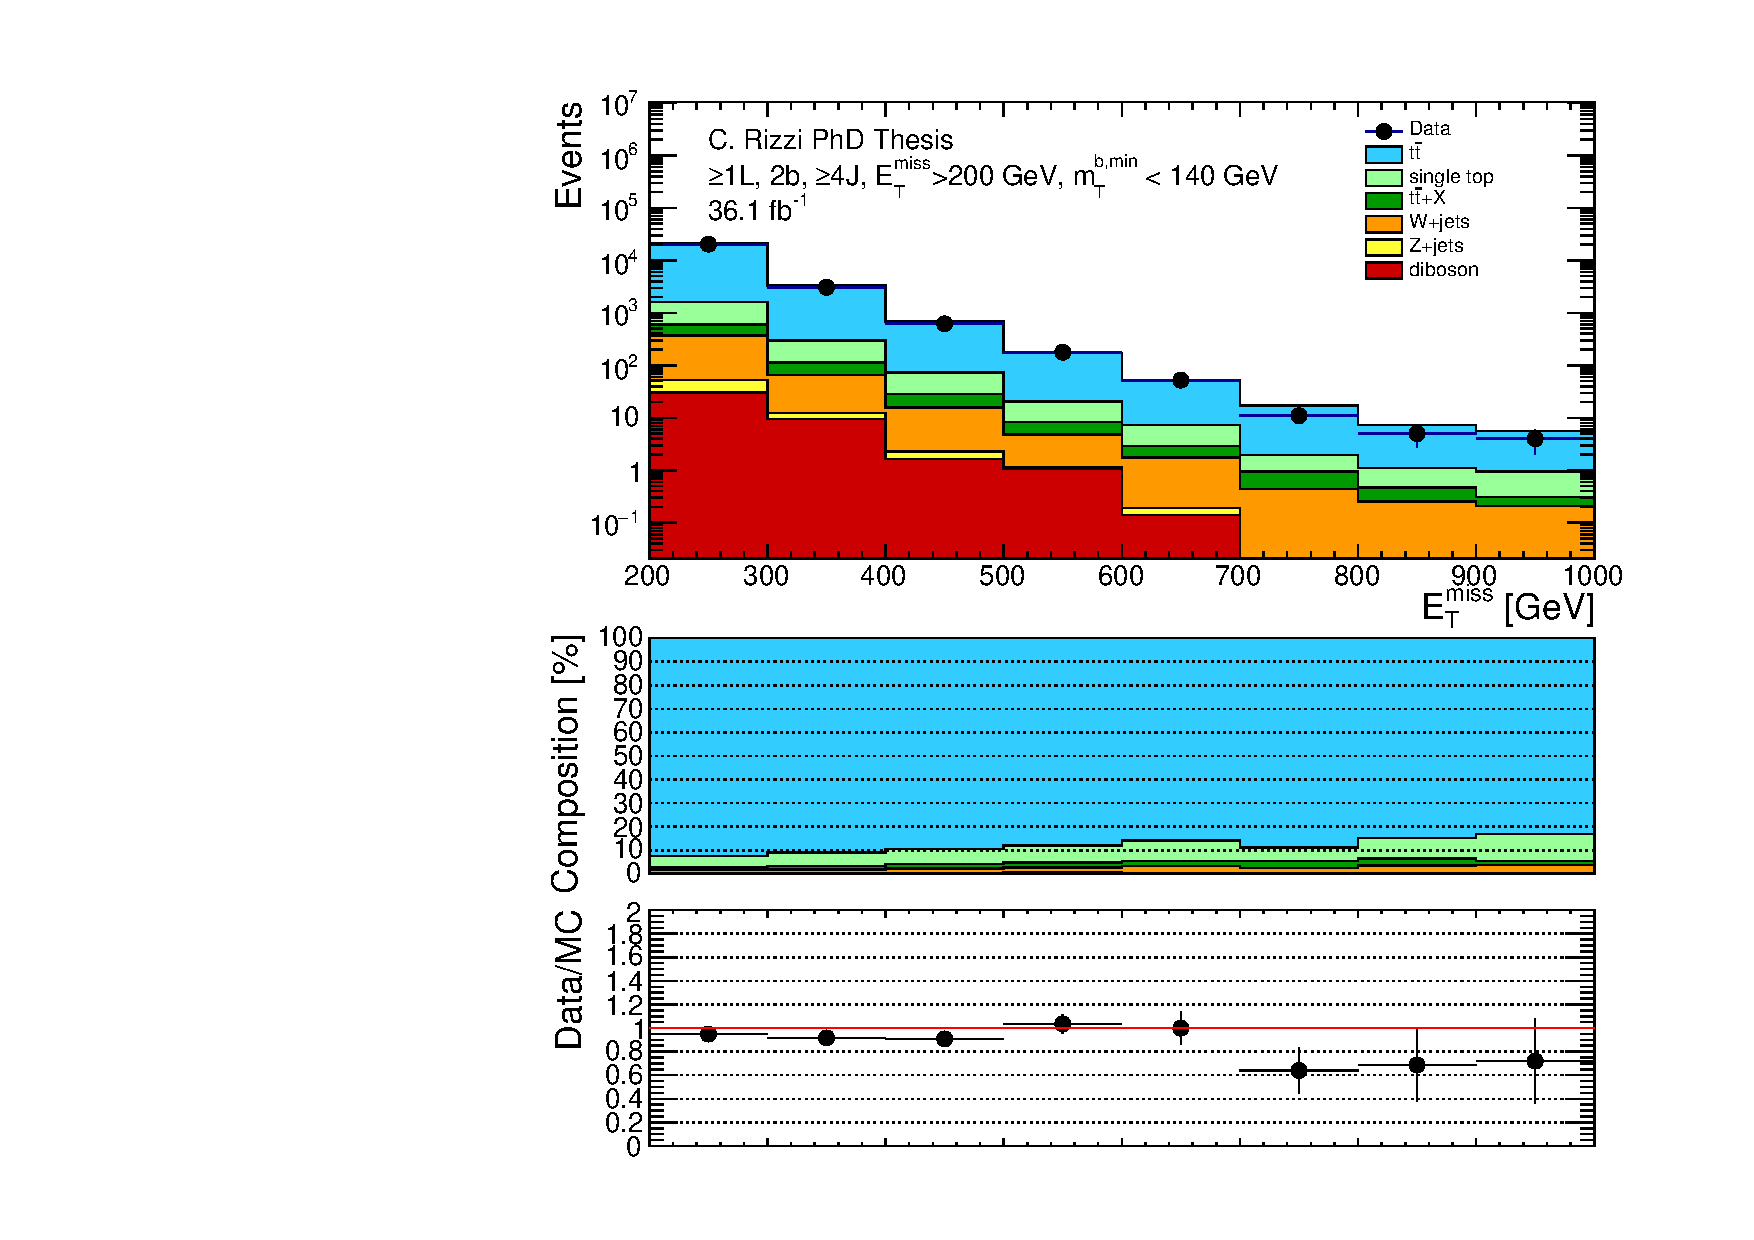
\includegraphics[width=0.45\textwidth]{figures/App1/Rizzi-FigA1-2-6.pdf}
\label{fig:strong:rwCR::datamc1L:met}}\\
\caption{Comparison between data and simulation in the reweighting region, before and after applying the kinematic reweighting.
}
\label{fig:strong:rwCR::datamc1L_a}
\end{figure*}

\begin{figure*}[htbp]
\centering 


\subfigure[\mt, before reweighting]{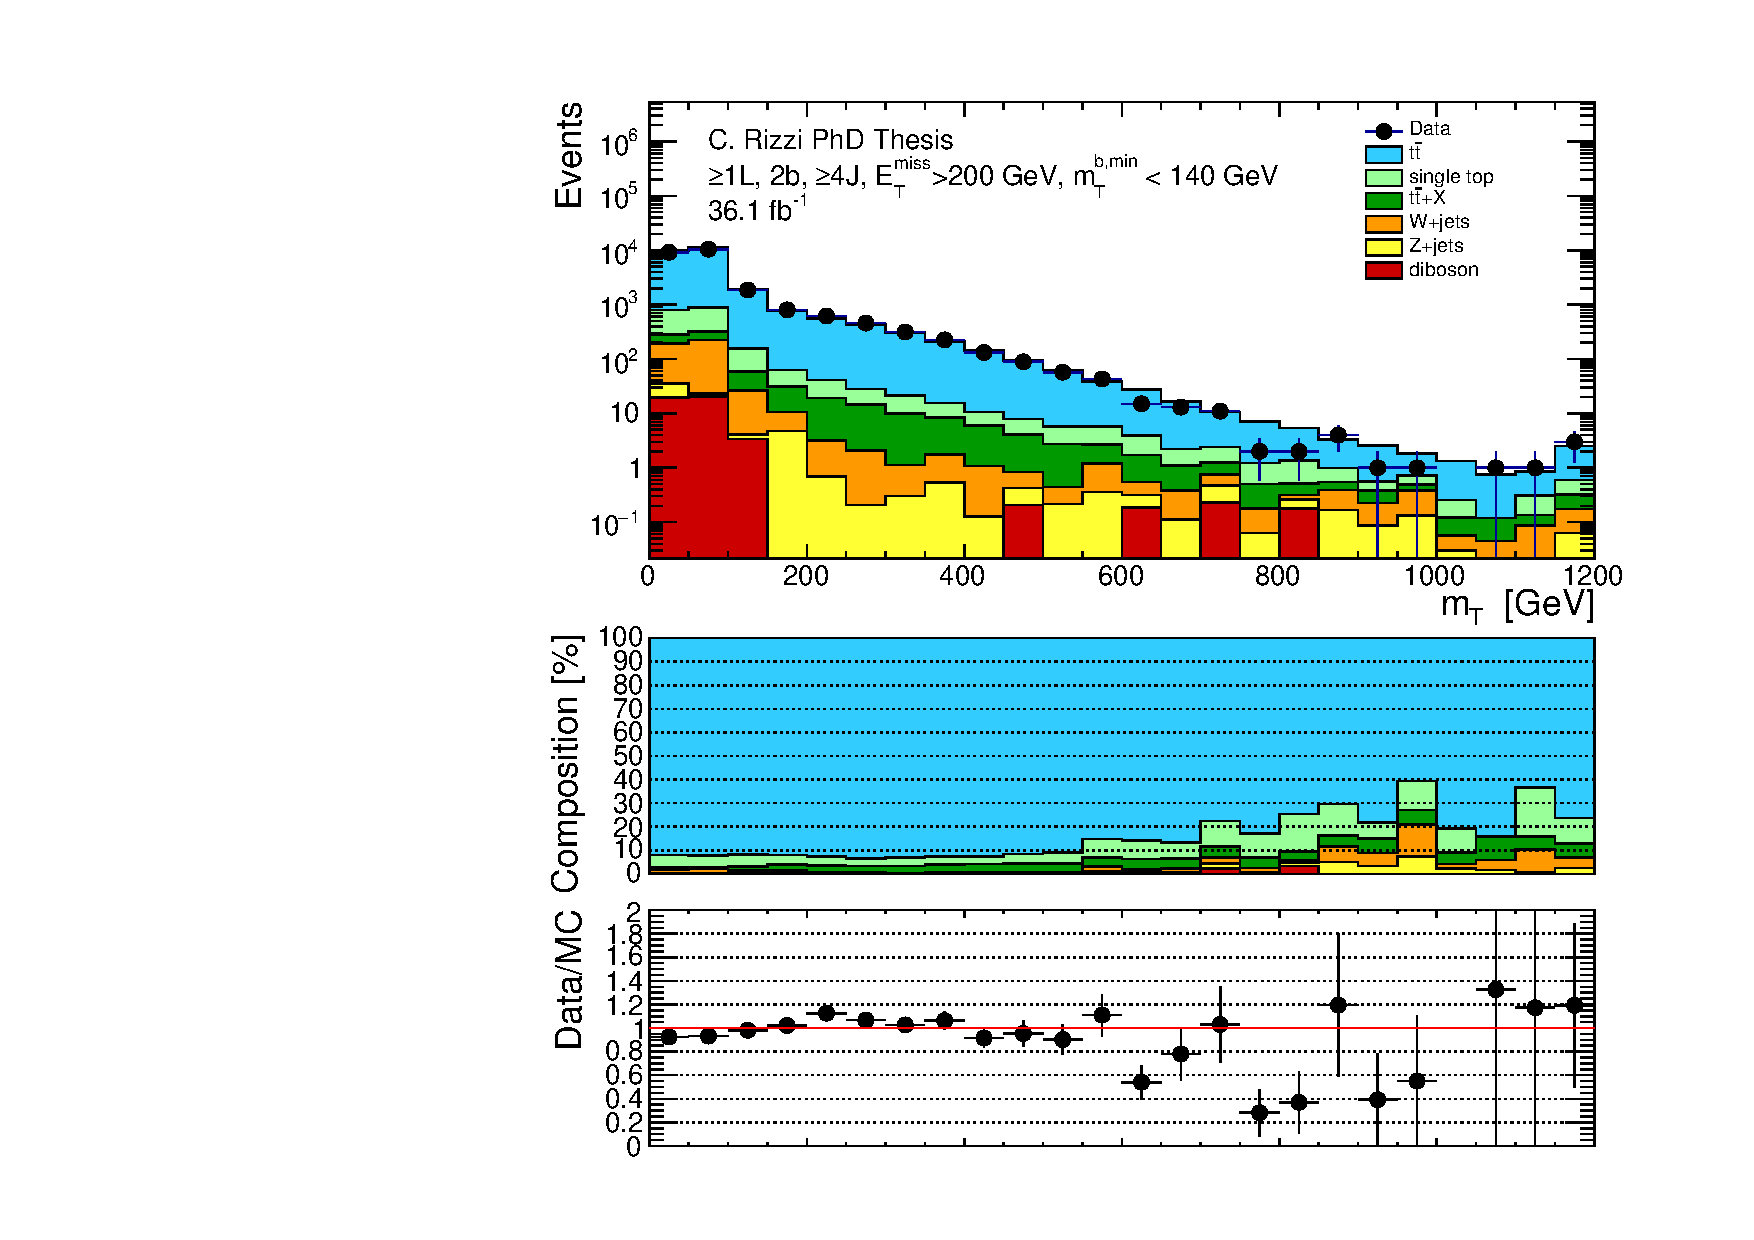
\includegraphics[width=0.45\textwidth]{figures/App1/Rizzi-FigA1-3-1.pdf}
\label{fig:strong:rwCR::datamc1L:mT}}
\subfigure[\mt, after reweighting]{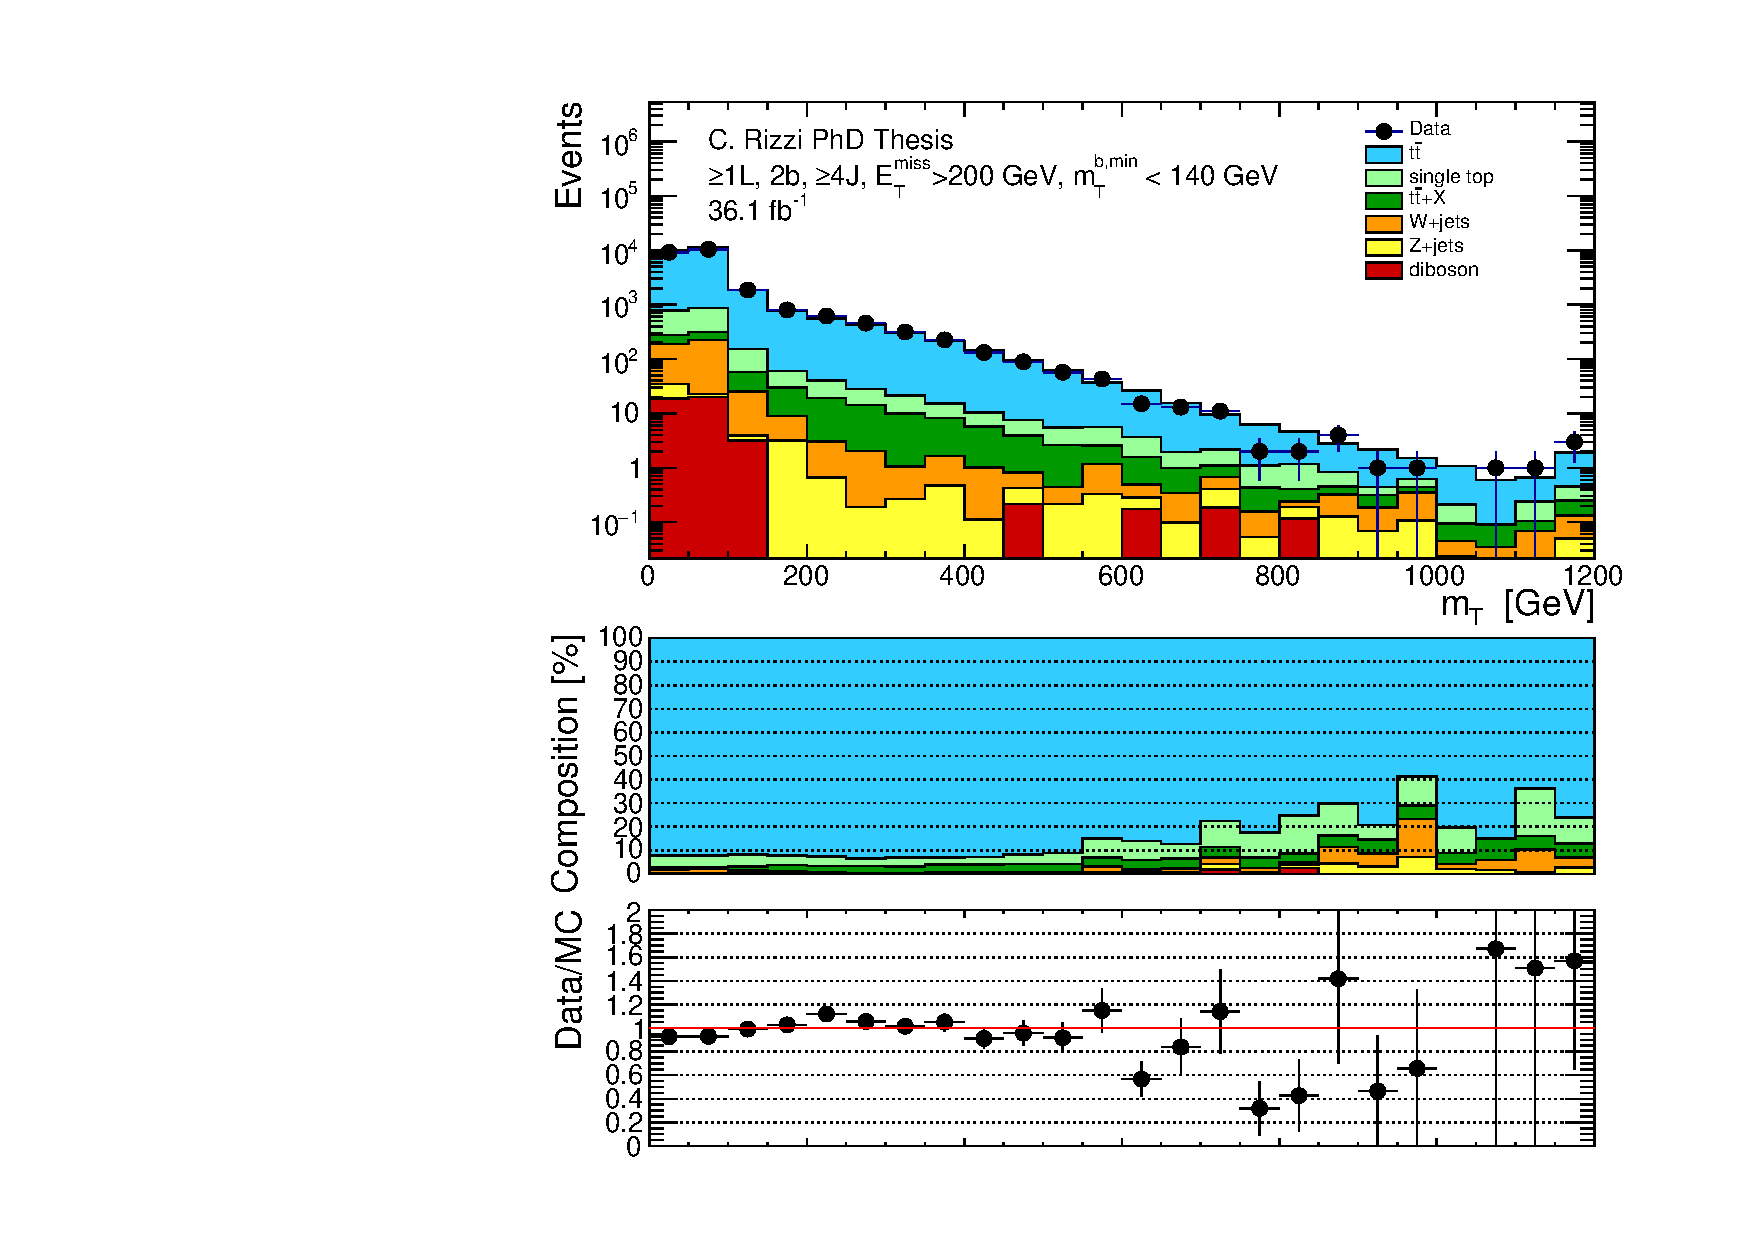
\includegraphics[width=0.45\textwidth]{figures/App1/Rizzi-FigA1-3-2.pdf}
\label{fig:strong:rwCR::datamc1L:mT}}\\
\subfigure[\njet, before reweighting]{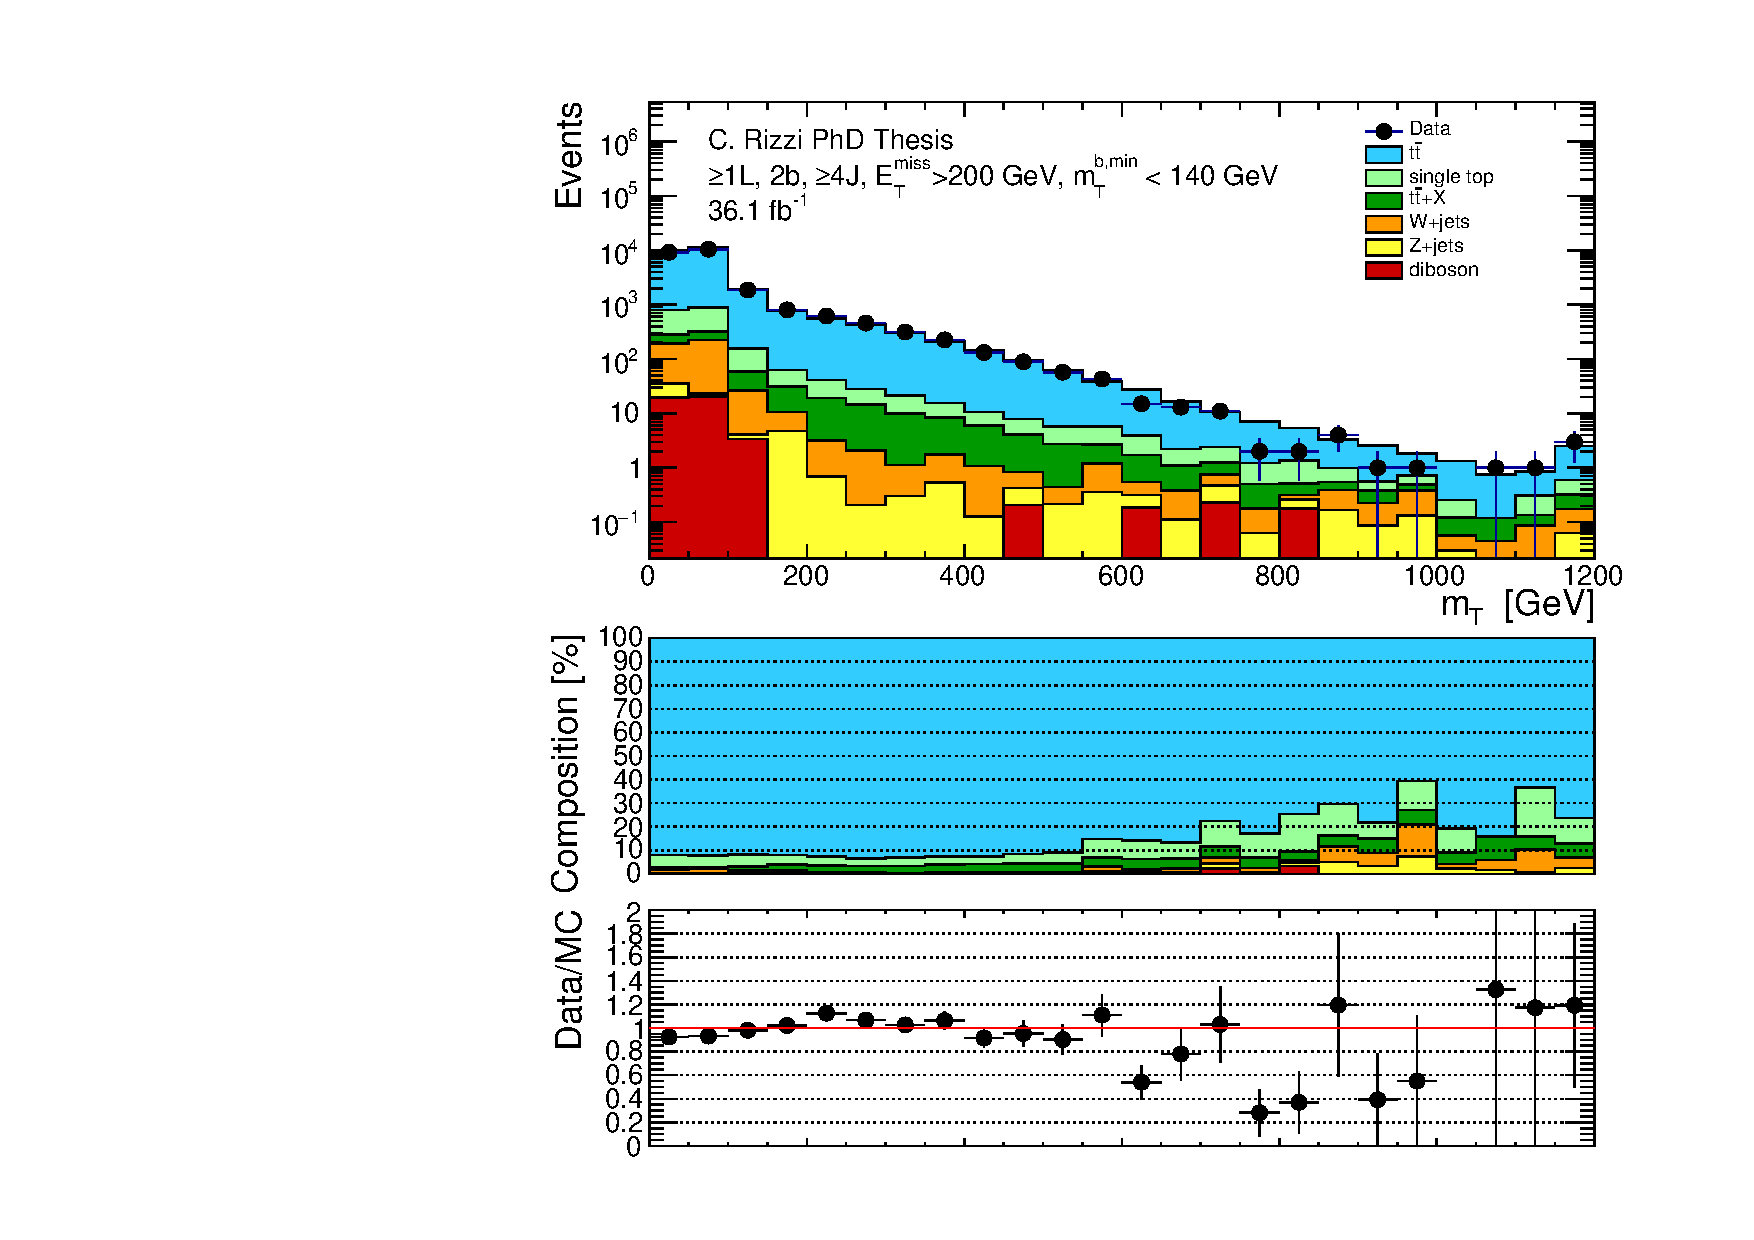
\includegraphics[width=0.45\textwidth]{figures/App1/Rizzi-FigA1-3-3.pdf}
\label{fig:strong:rwCR::datamc1L:jets_n}}
\subfigure[\njet, after reweighting]{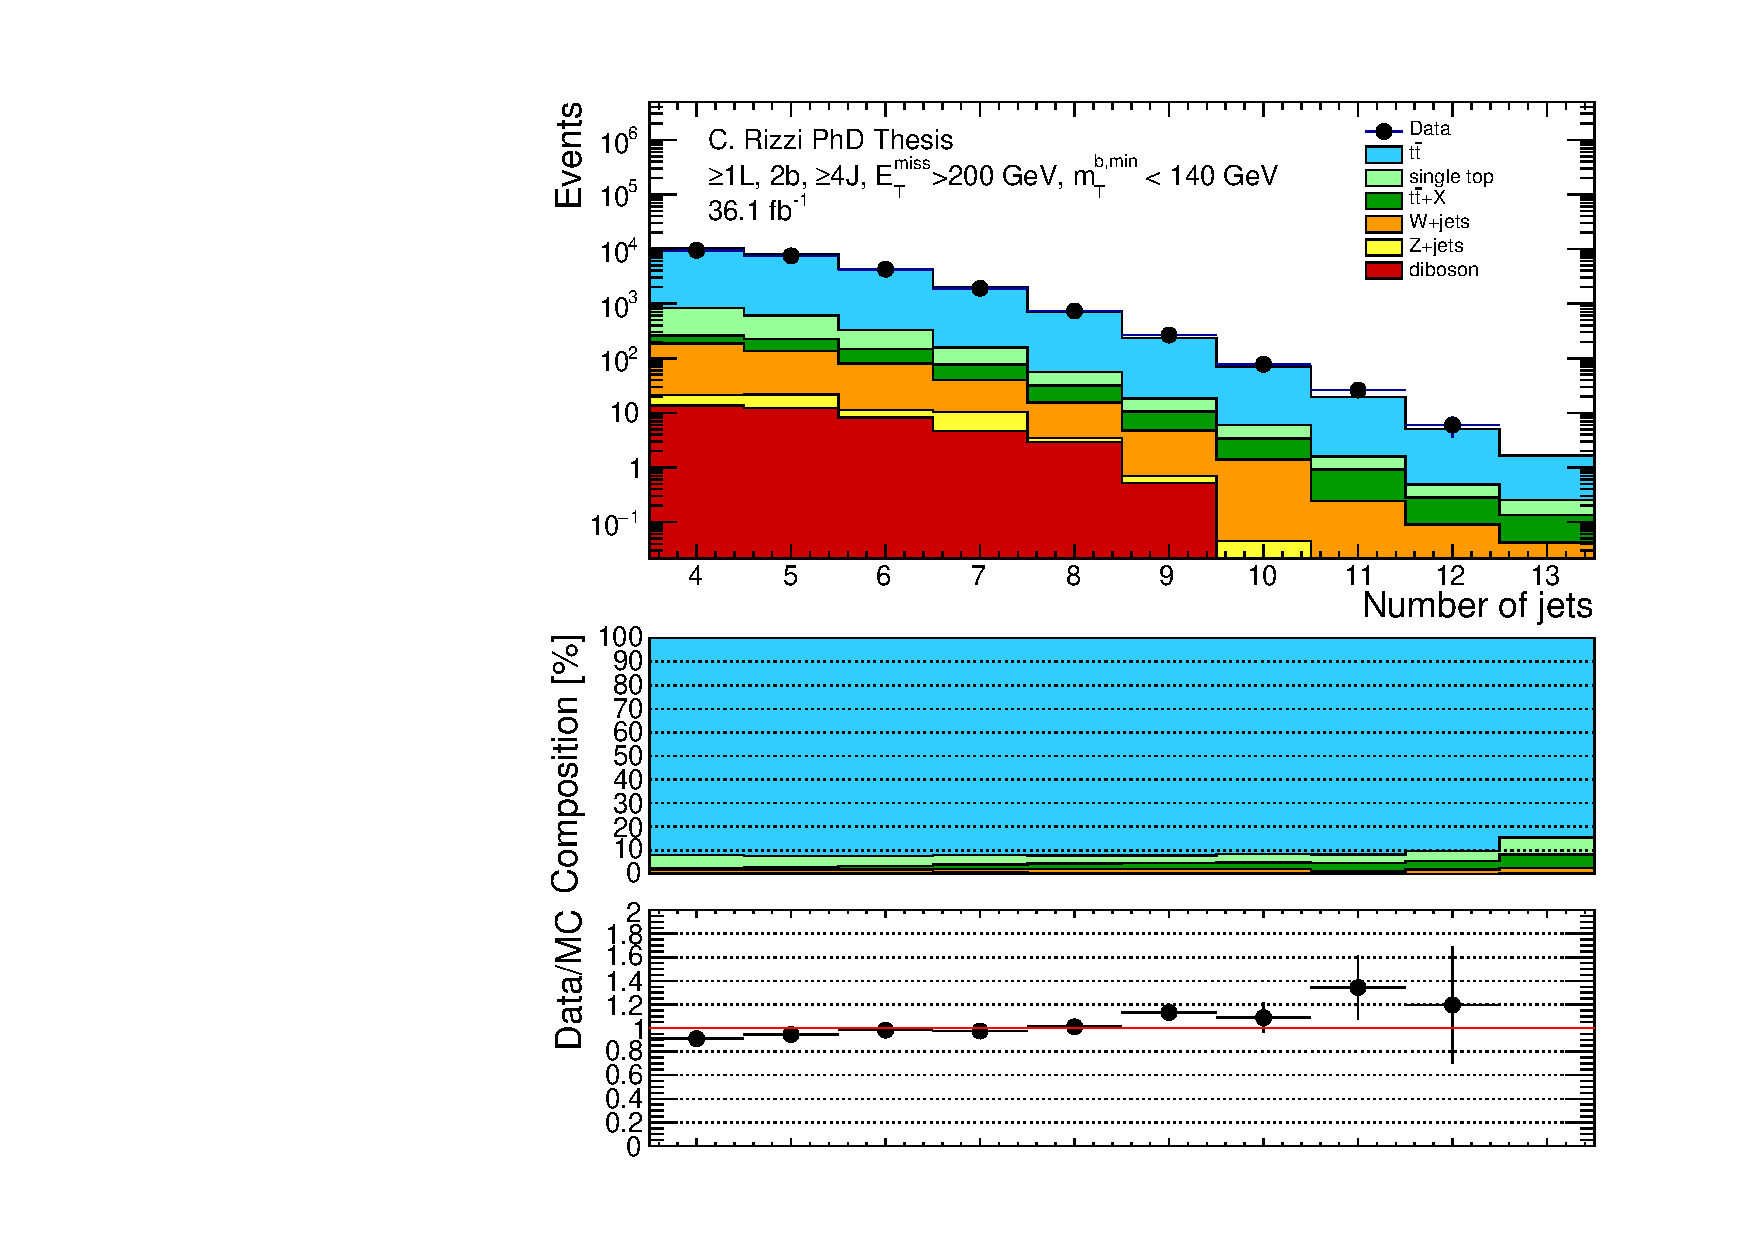
\includegraphics[width=0.45\textwidth]{figures/App1/Rizzi-FigA1-3-4.pdf}
\label{fig:strong:rwCR::datamc1L:jets_n}}\\
\subfigure[\pt jet$_1$, before reweighting]{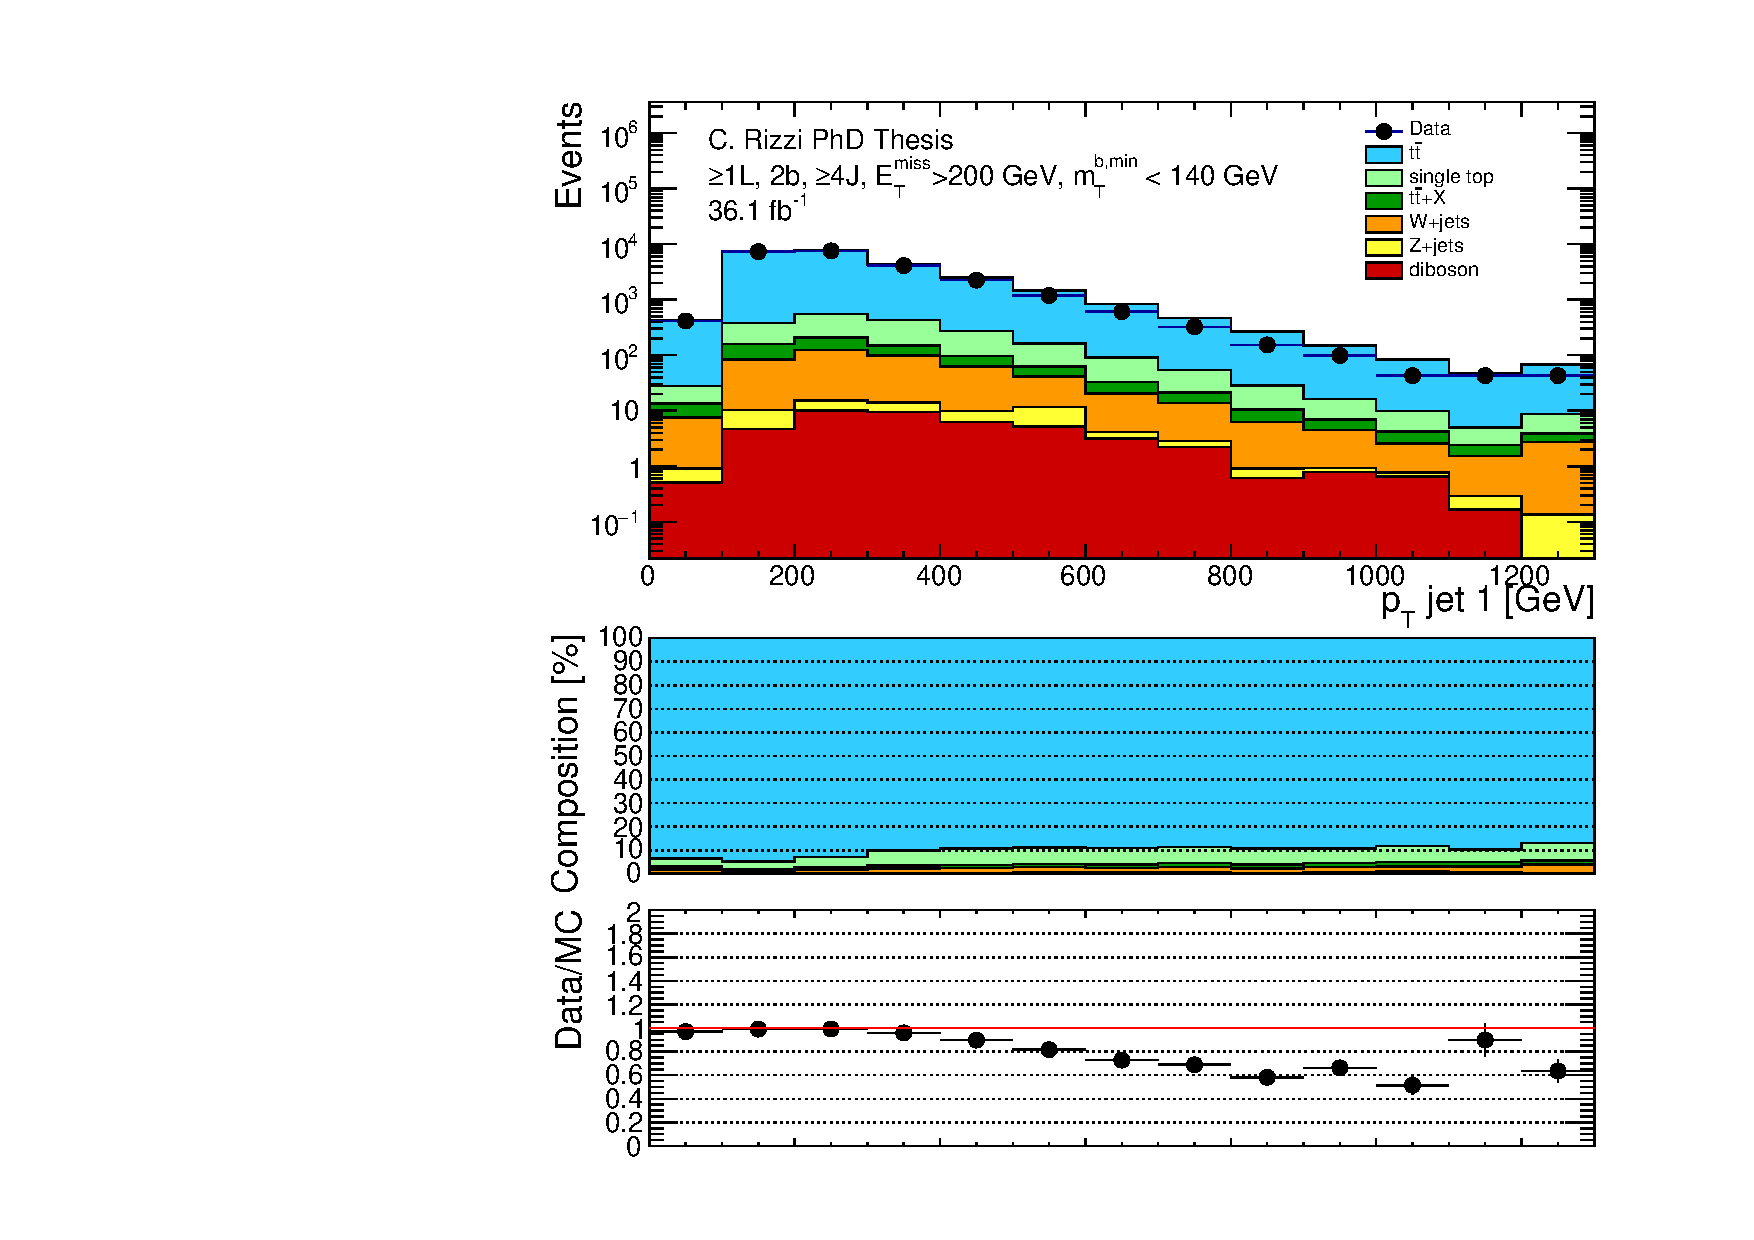
\includegraphics[width=0.45\textwidth]{figures/App1/Rizzi-FigA1-3-5.pdf}
\label{fig:strong:rwCR::datamc1L:pt_jet_1}}
\subfigure[\pt jet$_1$, after reweighting]{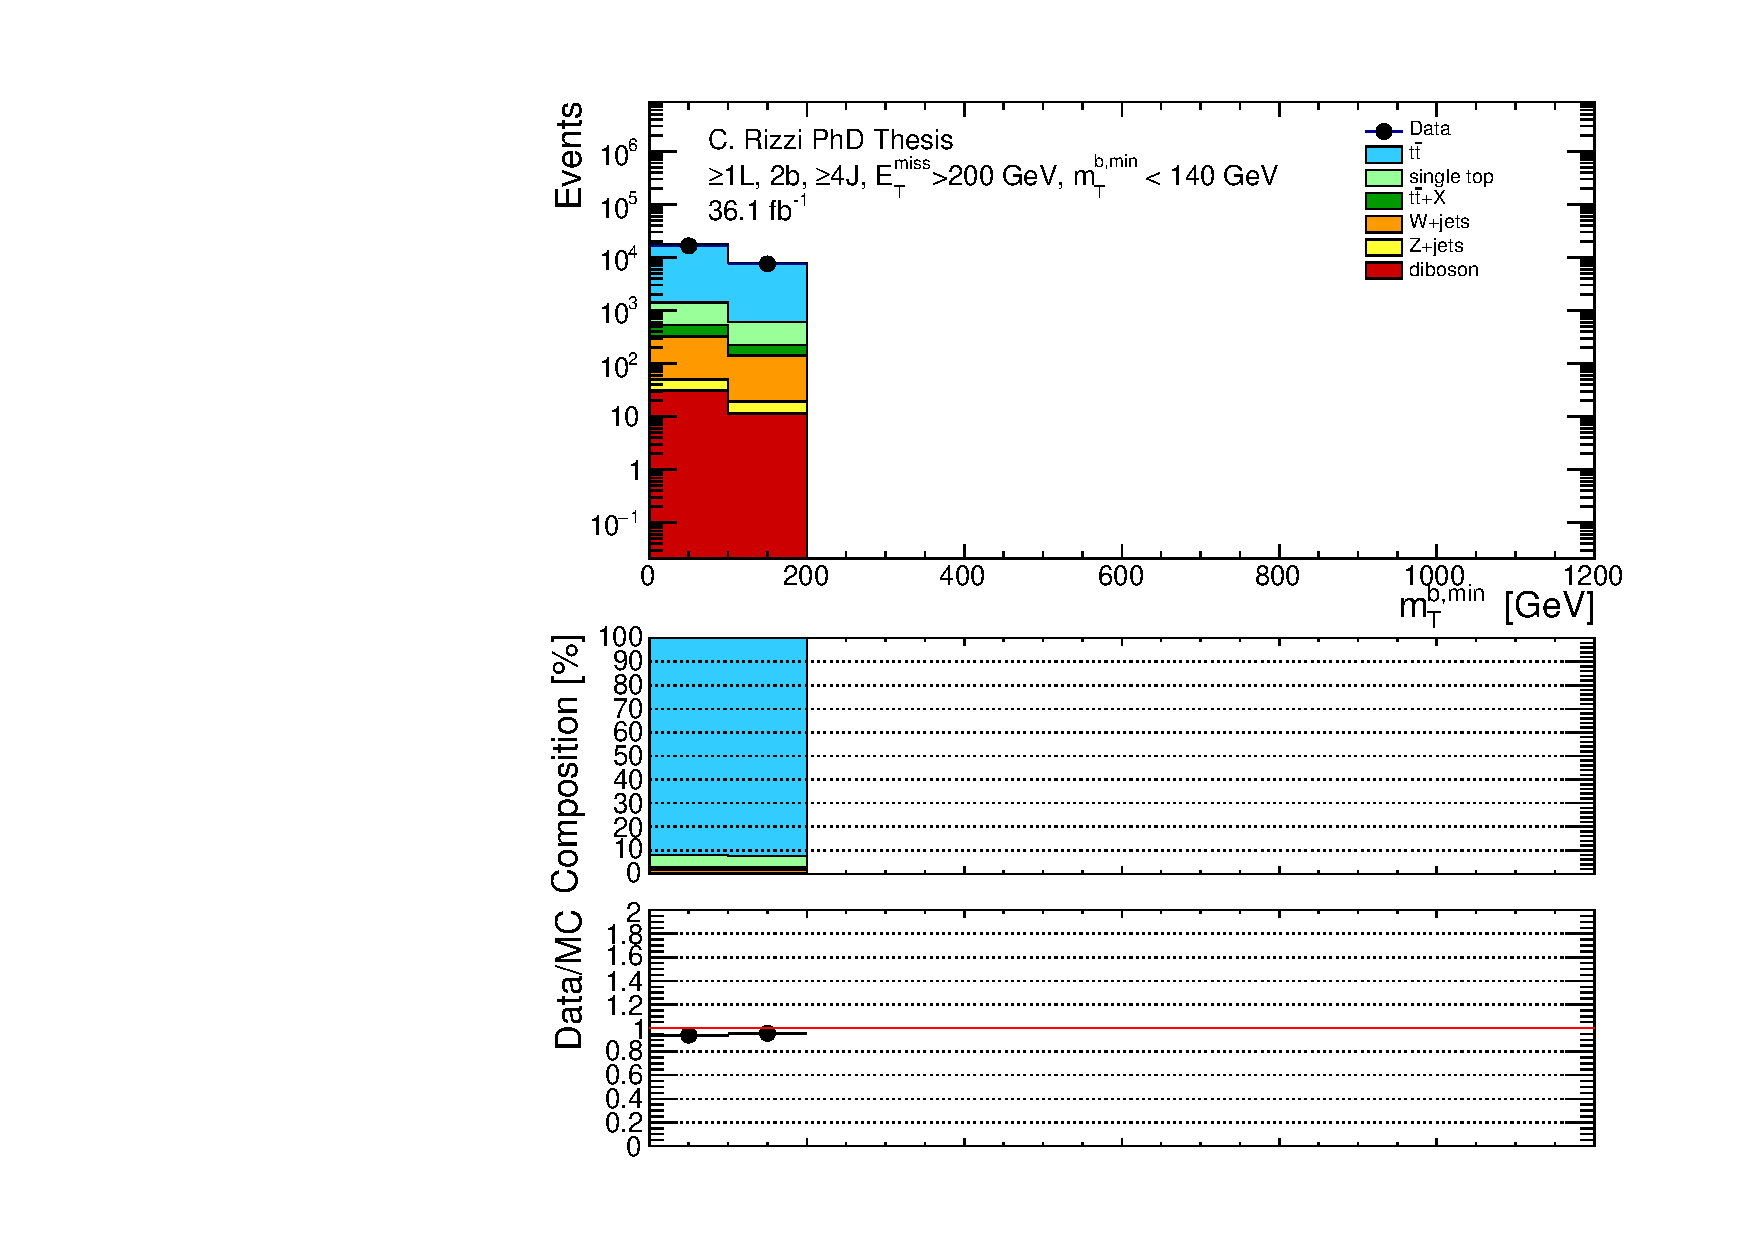
\includegraphics[width=0.45\textwidth]{figures/App1/Rizzi-FigA1-3-6.pdf}
\label{fig:strong:rwCR::datamc1L:pt_jet_1}}\\

\caption{Comparison between data and simulation in the reweighting region, before and after applying the kinematic reweighting.
}
\label{fig:strong:rwCR::datamc1L_b}
\end{figure*}

\begin{figure*}[htbp]
\centering 
\subfigure[\pt jet$_2$, before reweighting]{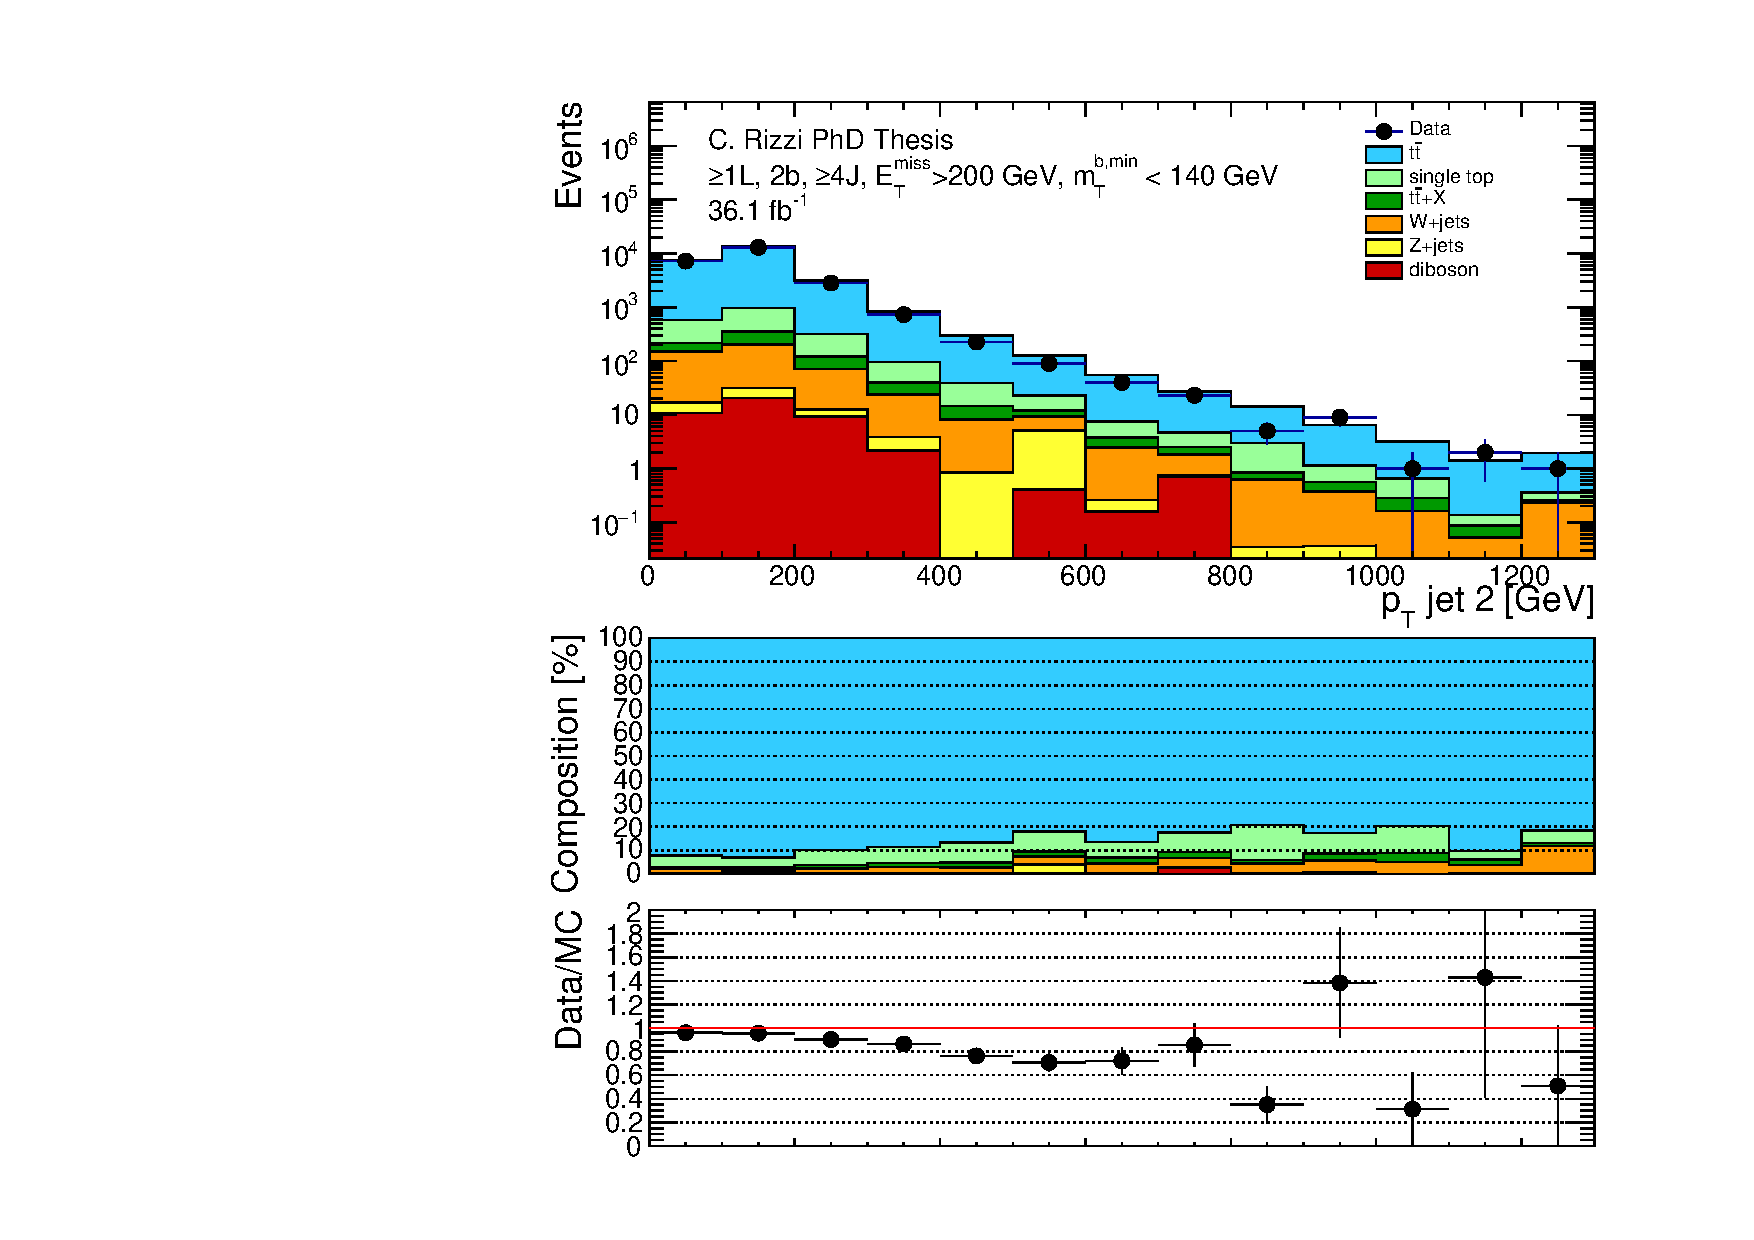
\includegraphics[width=0.45\textwidth]{figures/App1/Rizzi-FigA1-4-1.pdf}
\label{fig:strong:rwCR::datamc1L:pt_jet_2}}
\subfigure[\pt jet$_2$, after reweighting]{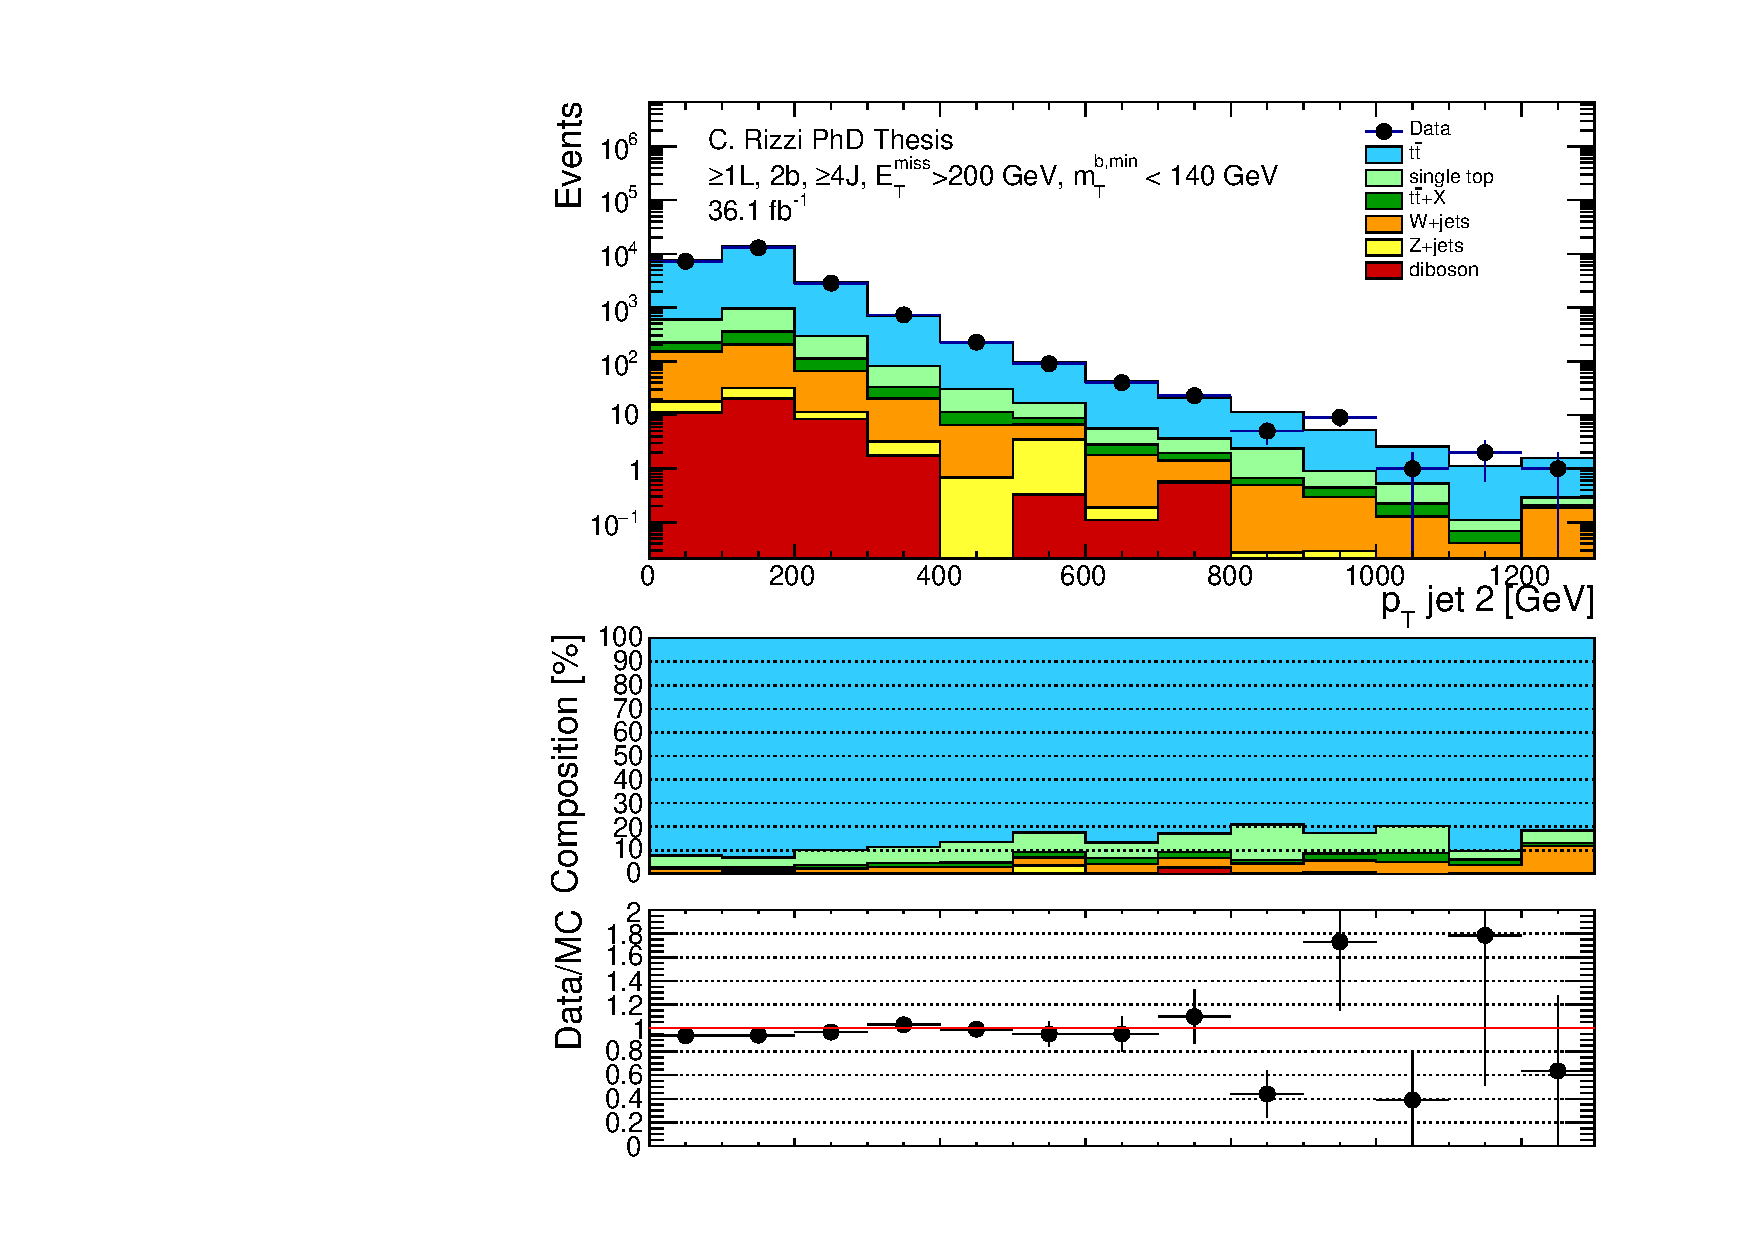
\includegraphics[width=0.45\textwidth]{figures/App1/Rizzi-FigA1-4-2.pdf}
\label{fig:strong:rwCR::datamc1L:pt_jet_2}}\\
\subfigure[\pt lep$_1$, before reweighting]{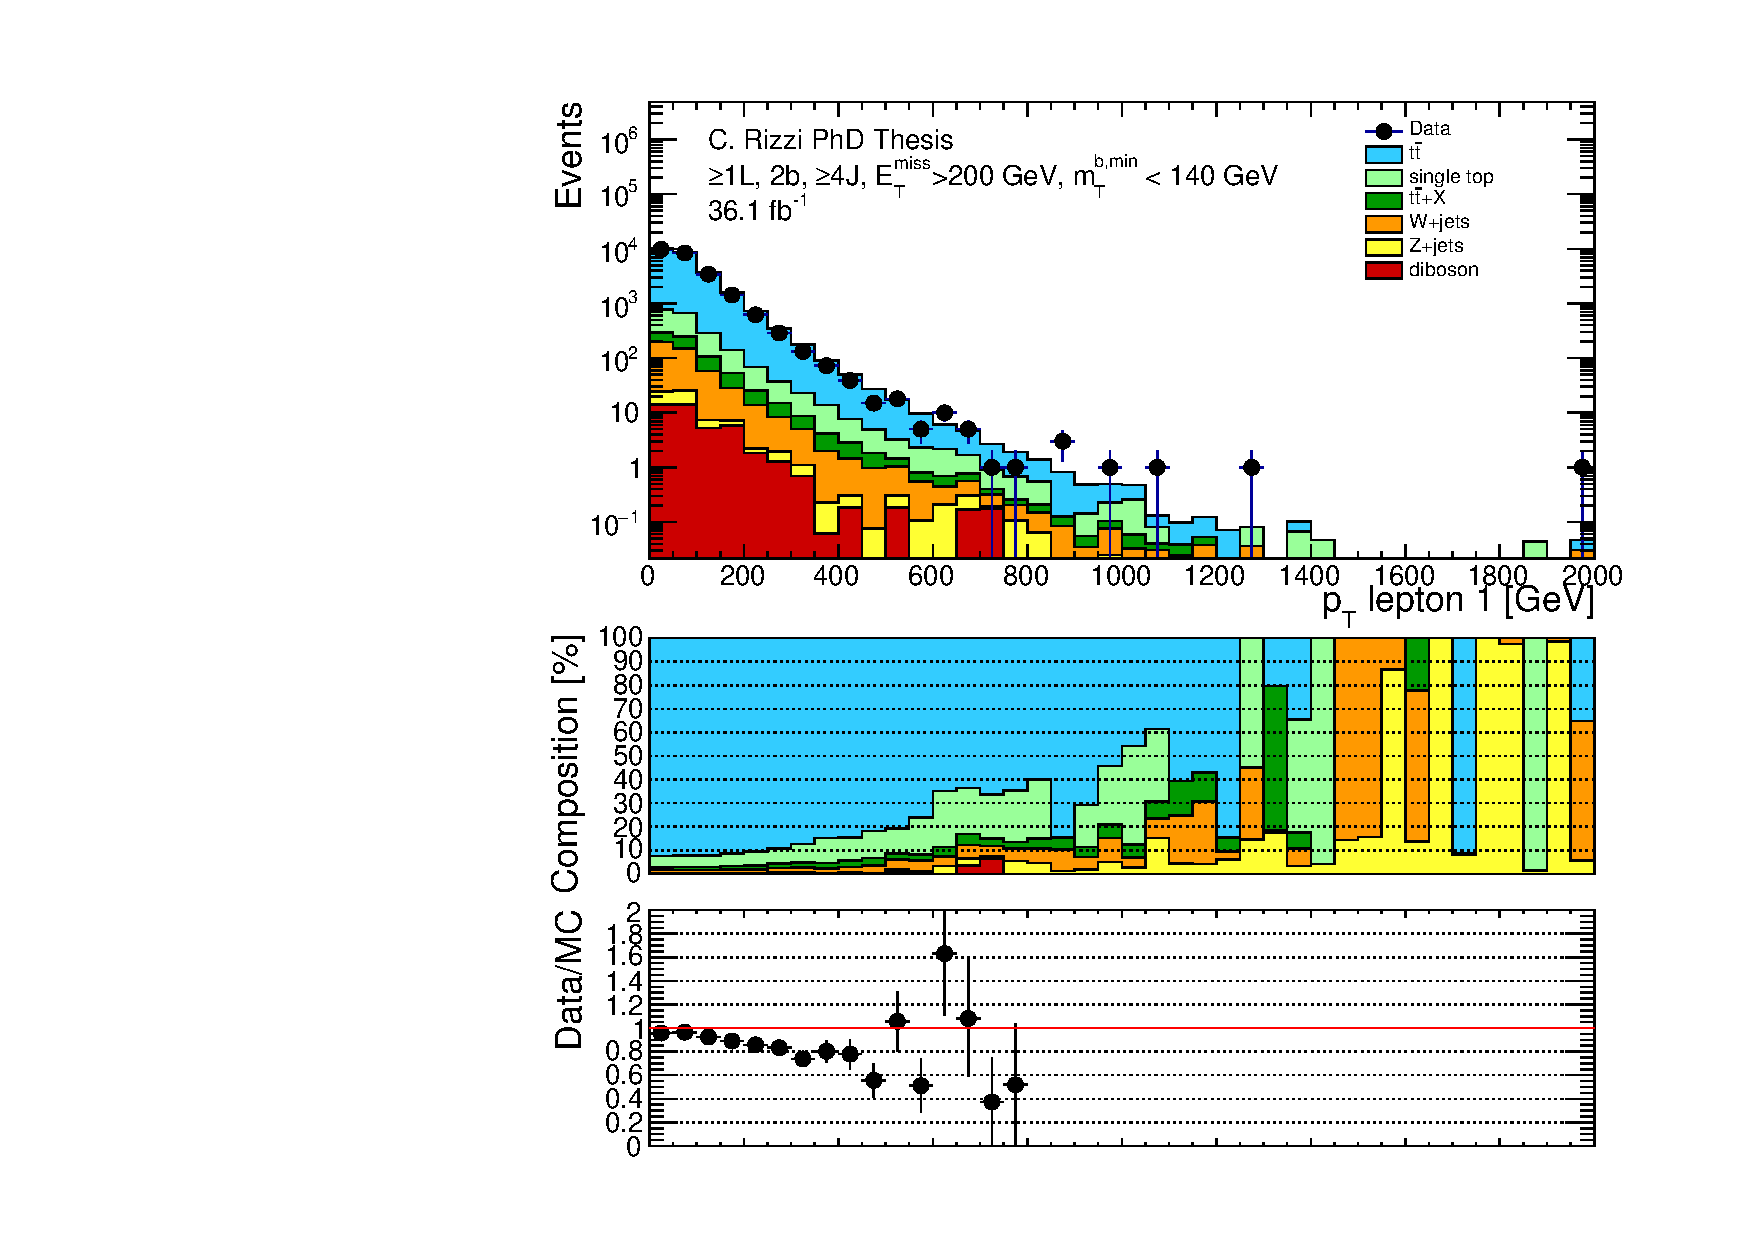
\includegraphics[width=0.45\textwidth]{figures/App1/Rizzi-FigA1-4-3.pdf}
\label{fig:strong:rwCR::datamc1L:ptlep1}}
\subfigure[\pt lep$_1$, after reweighting]{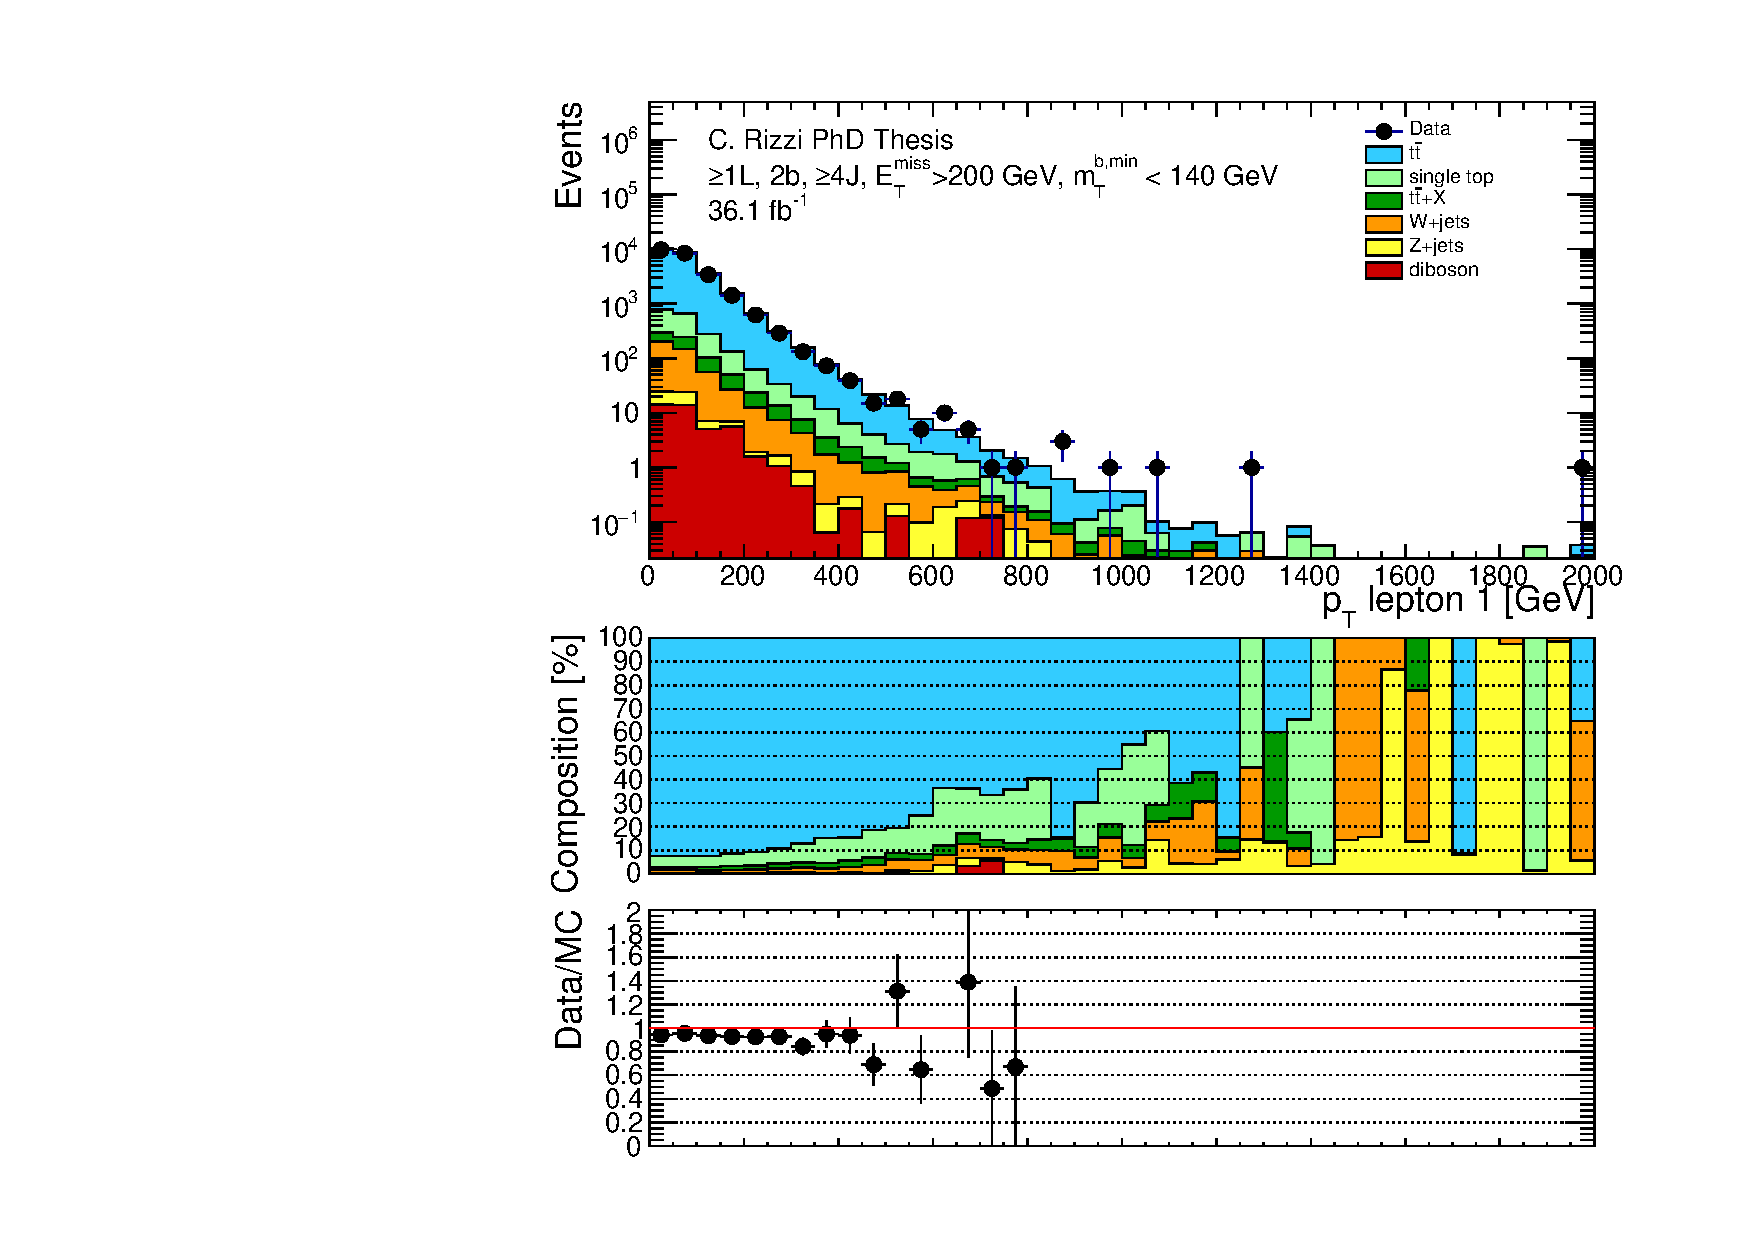
\includegraphics[width=0.45\textwidth]{figures/App1/Rizzi-FigA1-4-4.pdf}
\label{fig:strong:rwCR::datamc1L:ptlep1}}\\
\subfigure[\pt $b$-jet$_1$, before reweighting]{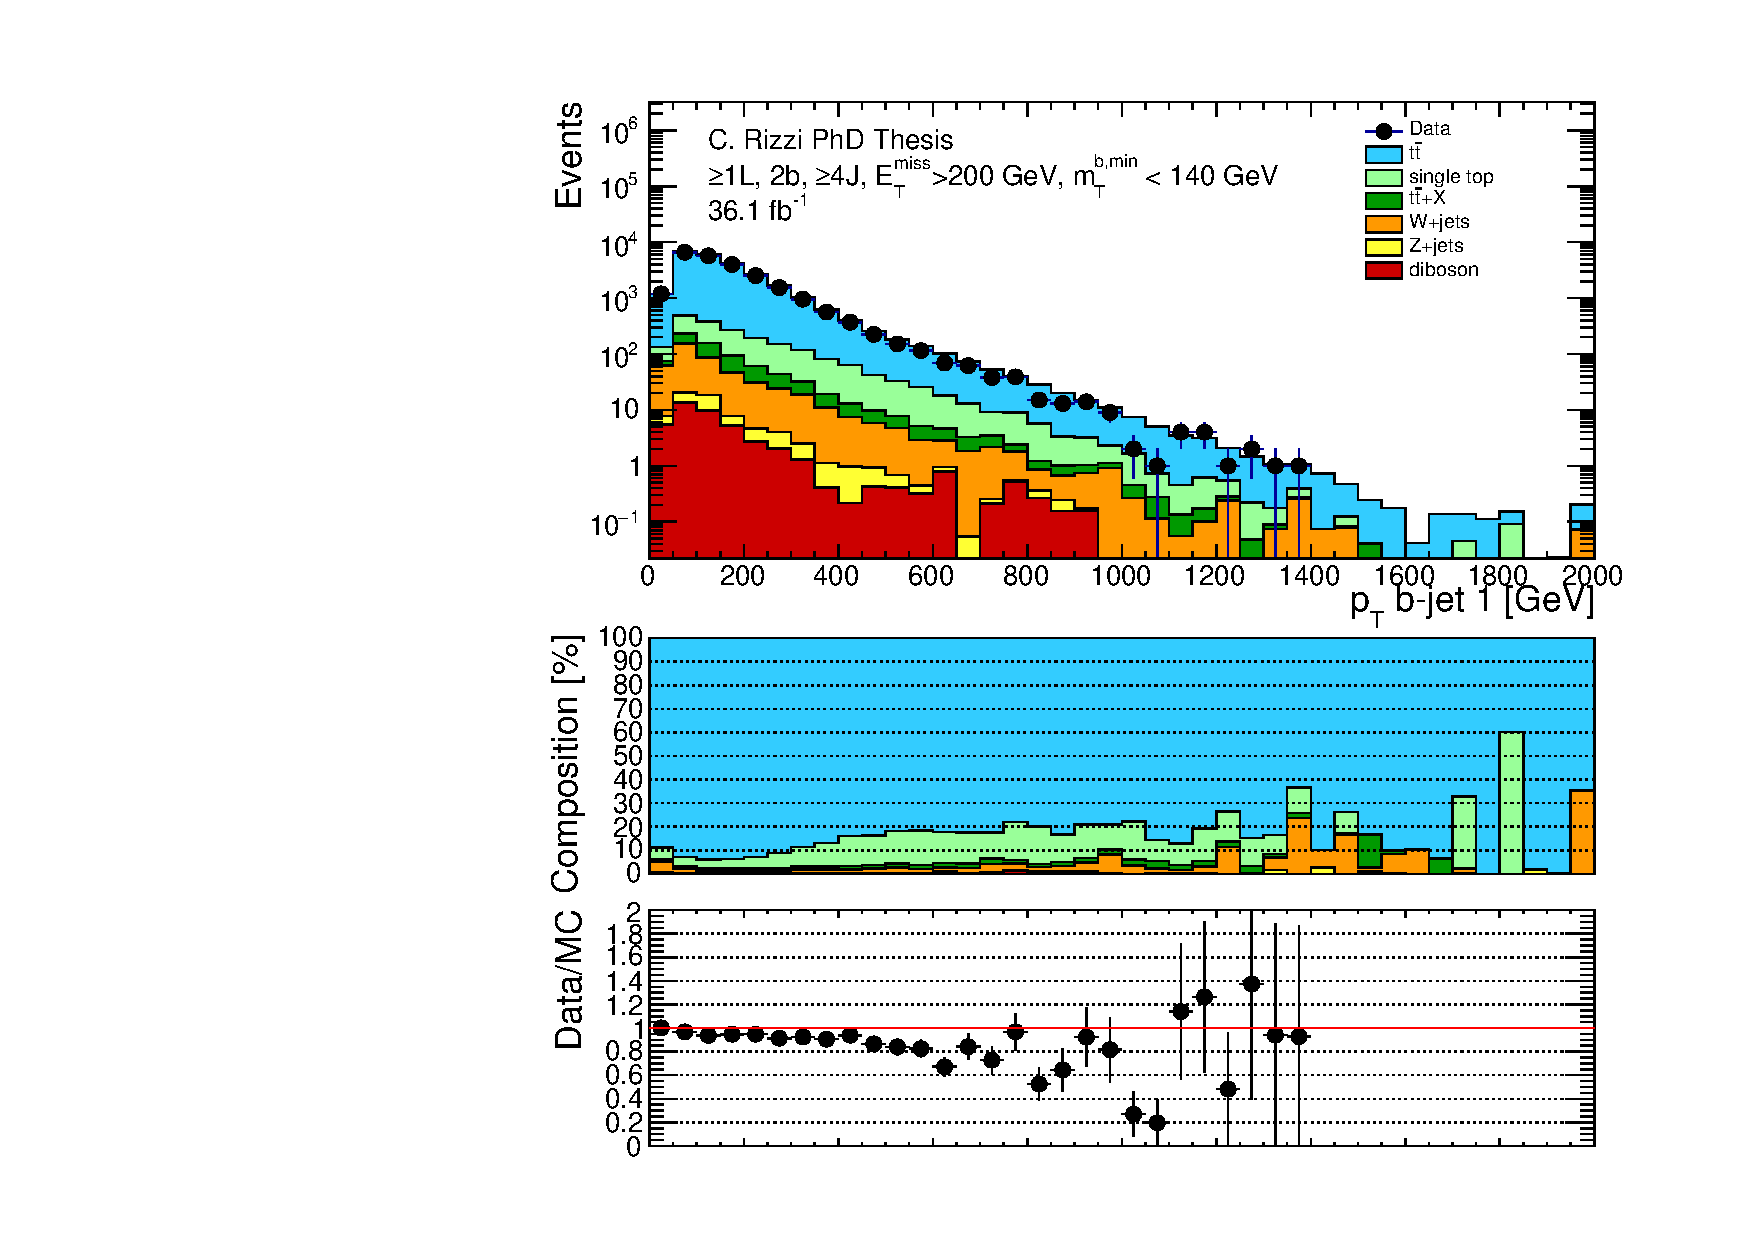
\includegraphics[width=0.45\textwidth]{figures/App1/Rizzi-FigA1-4-5.pdf}
\label{fig:strong:rwCR::datamc1L:pt_bjet_1}}
\subfigure[\pt $b$-jet$_1$, after reweighting]{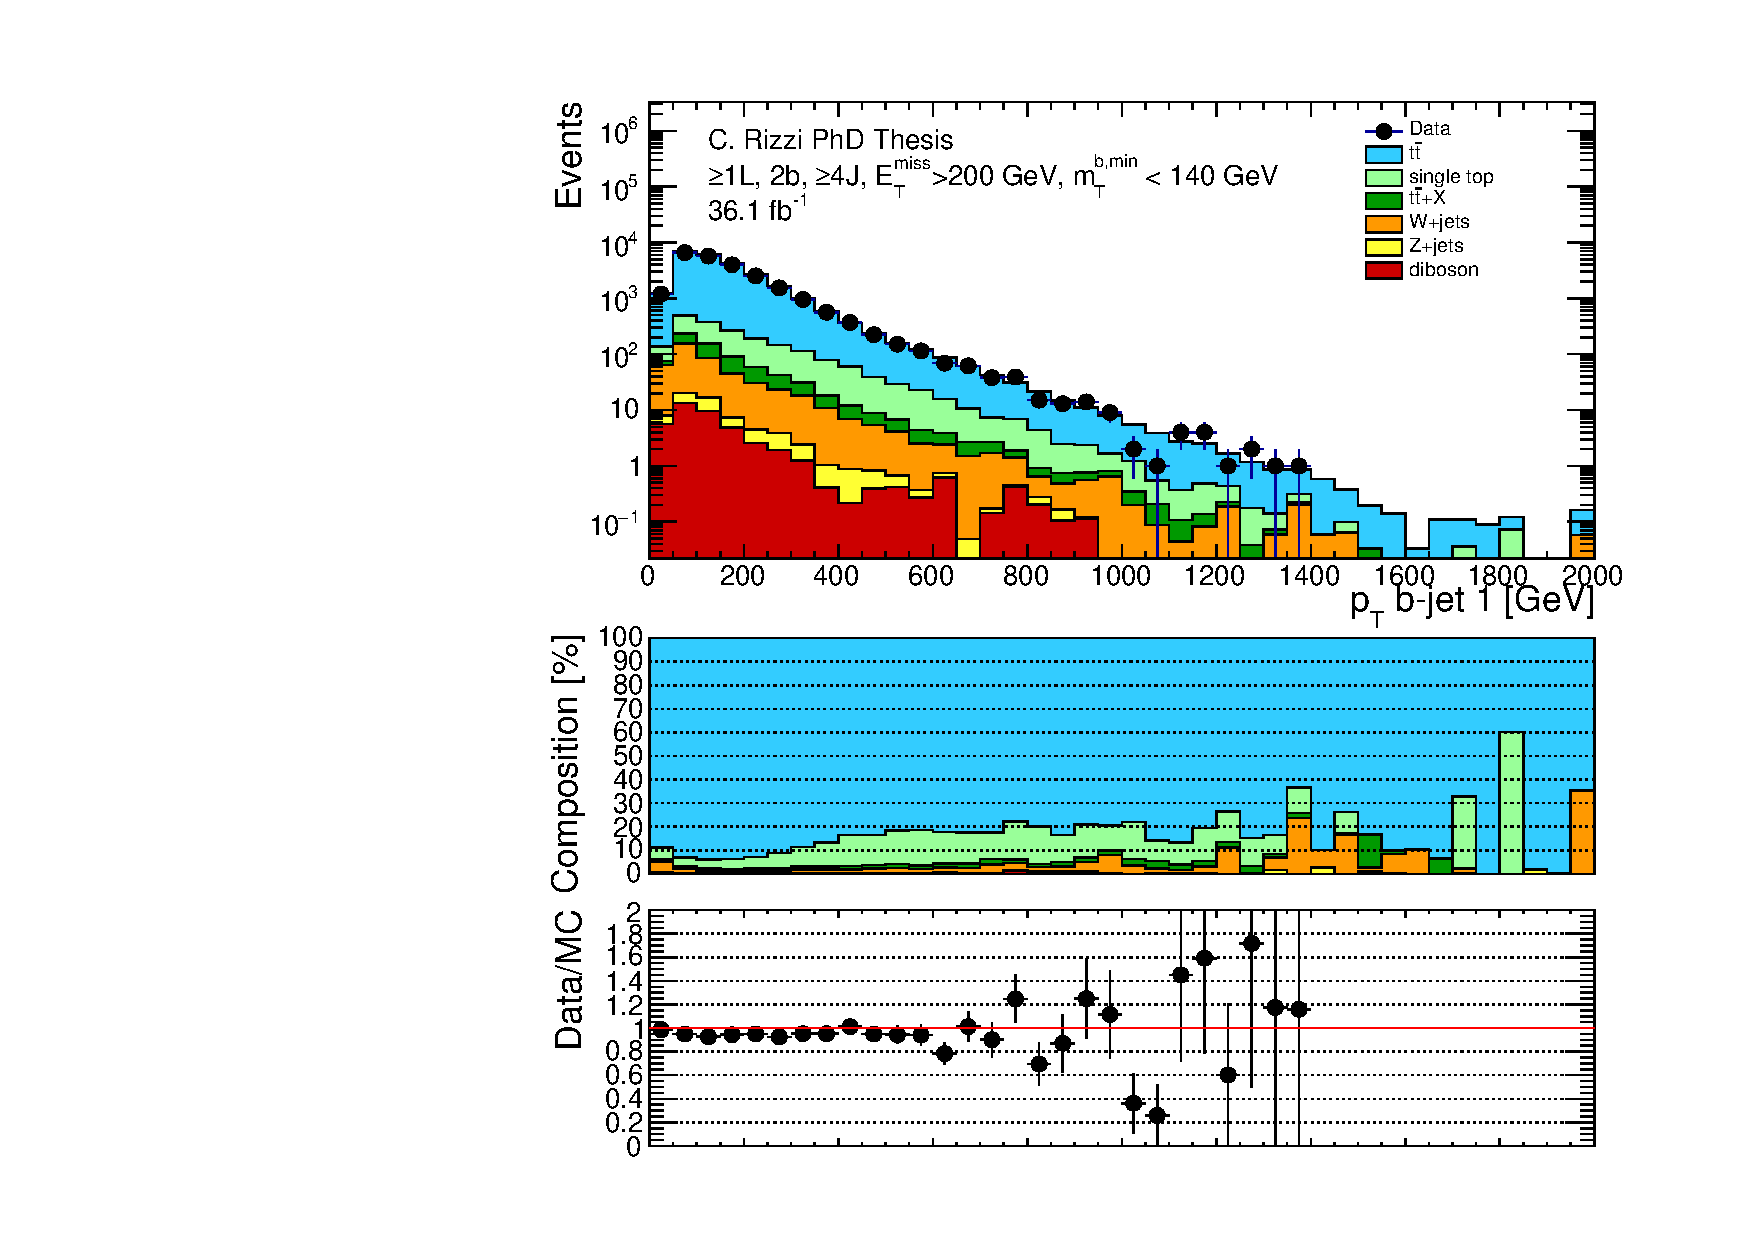
\includegraphics[width=0.45\textwidth]{figures/App1/Rizzi-FigA1-4-6.pdf}
\label{fig:strong:rwCR::datamc1L:pt_bjet_1}}
\caption{Comparison between data and simulation in the reweighting region, after applying the kinematic reweighting.
}
\label{fig:strong:rwCR::datamc1L_d}
\end{figure*}





